%%
%% This file follows the user's own elsarticle-template-num.tex, uploaded
%% for this project. Preamble, proof formatting, and frontmatter structure
%% are matched to that template; content (title, abstract, keywords, body)
%% is this paper's own.
\documentclass[final,5p,twocolumn]{elsarticle}

\usepackage{amsmath,amsfonts}
\usepackage{algorithm}
\usepackage{algpseudocode}
\renewcommand{\Comment}[1]{\hfill$\triangleright$ #1}
\usepackage{array}
\usepackage[font=normalsize,labelfont=bf]{caption}
\usepackage[]{subcaption}
\usepackage{arydshln}
\usepackage{textcomp}
\usepackage{stfloats}
\usepackage{url}
\usepackage{verbatim}
\usepackage{graphicx}
\usepackage{IEEEtrantools}
\usepackage{hyperref}
\usepackage{setspace}
\usepackage{soul}
\usepackage{xcolor}
\usepackage{bm}
\usepackage{amsthm}
\hyphenation{op-tical net-works semi-conduc-tor IEEE-Xplore}
\def\BibTeX{{\rm B\kern-.05em{\sc i\kern-.025em b}\kern-.08em
		T\kern-.1667em\lower.7ex\hbox{E}\kern-.125emX}}
\usepackage{balance}
\setlength{\textfloatsep}{8pt}
\newcommand{\orcidlink}[1]{\href{https://orcid.org/#1}{\includegraphics[scale=0.06]{pictures/orcid.png}}}

\newtheorem{definition}{Definition}
\newtheorem{lemma}{Lemma}
% The template defines Definition and Lemma only; Corollary and Remark are
% this paper's own addition, chained to the same counter as Lemma so all
% three number in one sequence through the appendix.
\newtheorem{corollary}[lemma]{Corollary}
\theoremstyle{remark}
\newtheorem{remark}{Remark}
\theoremstyle{plain}

\raggedbottom
\makeatletter
\usepackage{xcolor,etoolbox}
\makeatletter
\renewcommand\proofname{\textcolor{black}{\textbf{Proof}}}

\patchcmd{\proof}
{\item[\hskip\labelsep\scshape #1\@addpunct{.}]}
{\item[\hskip\labelsep\bfseries\color{black}#1\@addpunct{:}] \mbox{}\\}
{}{}%

\patchcmd{\proof}
{\item[\hskip\labelsep #1\@addpunct{.}]}
{\item[\hskip\labelsep\bfseries\color{black}#1\@addpunct{:}] \mbox{}\\}
{}{}%

\patchcmd{\proof}
{\item[\hskip\labelsep\textit{#1}\@addpunct{.}]}
{\item[\hskip\labelsep\bfseries\color{black}#1\@addpunct{:}] \mbox{}\\}
{}{}%
\makeatother
\renewcommand{\qedsymbol}{}

\newcommand{\TBD}{\textbf{TBD}} % placeholder for the one confirmed unrun analysis (density sweep); real results go in directly elsewhere

\journal{Journal of Network and Computer Applications}

\begin{document}

\begin{frontmatter}

\title{Post Quantum Mobility Adaptive Zero Trust Detection of Selective Time Delay Attacks via STARK Timing Attestation, ML-DSA-87 Aggregate Signatures, and Controller Failover Blockchain Quarantine in Software Defined Vehicular Networks}

% TODO: author block pending confirmation of the final author list for this
% specific paper (distinct author ordering may apply versus VANGUARD-HF and
% NEXUS). Single author set below, matching the pattern of the uploaded
% template with its own co-author block commented out.
\author[1]{Patikiri Arachchige Don Shehan Nilmantha Wijesekara\orcidlink{0000-0002-3045-1596}\corref{cor1}}
\ead{nilmantha@eie.ruh.ac.lk}
\cortext[cor1]{Corresponding author: \texttt{nilmantha@eie.ruh.ac.lk}}

\affiliation[1]{organization={Department of Electrical \& Information Engineering, Faculty of Engineering, University of Ruhuna},
            city={Galle},
            postcode={80000},
            country={Sri Lanka}}

\begin{abstract}
	The centralized programmability of software defined vehicular networks
	exposes safety critical traffic to selective time delay attacks, in
	which a compromised controller, roadside unit, or vehicle delays
	priority packets such as collision avoidance warnings while ordinary
	traffic proceeds normally, causing dependent systems to act on stale
	data. Existing defenses calibrate a detection threshold once and hold
	it fixed, so legitimate handoff induced latency under realistic
	vehicular mobility routinely falls inside that fixed margin regardless
	of whether an attack is present; separately, every defense reviewed
	here trusts the controller issuing flow rules, providing no protection
	once the controller itself is compromised. This paper presents
	PHANTOM, a mobility adaptive, zero trust framework spanning a dual
	mode detection engine that adjusts its threshold to current vehicle
	density and speed, a post quantum timing attestation proof certifying
	delay compliance without revealing a vehicle's true timing, and a
	delay evidence trust channel that penalizes a timing manipulating
	controller even when every flow rule it issues remains authorized.
	Evaluated across attack penetration, vehicular speed to one hundred
	forty kilometers per hour, network scale, and decreasing observable
	evidence, PHANTOM sustains a macro Matthews correlation coefficient of
	$0.71$ at the default operating point against $0.37$ for the strongest
	baseline, with end to end
	latency within the hundred millisecond safety bound throughout. These
	results show that a threshold calibrated to the mobility condition it
	operates under, combined with zero trust extended to the controller
	itself, closes a gap neither mobility unaware nor controller trusting
	defenses close alone.
\end{abstract}

\begin{keyword}
	Software Defined Vehicular Networks \sep Selective Time Delay Attack \sep Post Quantum Cryptography \sep Zero Trust Architecture \sep Mobility Aware Detection \sep Blockchain
\end{keyword}

\end{frontmatter}

\section{Introduction}\label{introduction}

\subsection{Background}

\IEEEPARstart{S}{oftware} defined vehicular networks decouple traffic forwarding at
roadside units from routing decisions made by a logically centralized
controller, enabling flexible flow management across a rapidly changing
vehicular topology. This same programmability creates an attack surface
absent from static deployments: a compromised controller, roadside unit,
or vehicle can selectively delay safety critical packets, such as
collision avoidance warnings, while ordinary traffic continues to flow
normally, so the attack mimics legitimate behaviour closely enough that a
detector watching only for volume or outright packet loss never sees it.
This paper addresses this attack class, selective time delay, as one of
two disjoint classes this project considers, the other being hidden
forwarding, developed independently in the companion paper VANGUARD HF
\cite{VanguardHF2026}.

Trust and intrusion detection in vehicular networks predate software
defined integration entirely, and the transition does not remove that
earlier work's relevance so much as expose what it never had to consider.
Early lightweight intrusion detection mechanisms for vehicular networks
targeted denial of service, integrity violation, and false alert
generation at the application layer, using cooperative guard vehicles and
a reputation schema to evaluate trust \cite{Sedjelmaci2014}, and hardware
backed chains of trust built on direct anonymous attestation addressed
message authenticity and privacy before any centralized controller existed
to compromise \cite{Sumra2011}. Once a centralized controller is
introduced, it becomes a concrete, demonstrated target in its own right: a
topology poisoning attack has been successfully carried out against four
mainstream software defined controllers under realistic vehicular
mobility, showing that the controller's own view of the network can be
corrupted directly rather than only the traffic it manages
\cite{Wang2020Topology}. Blockchain has separately been proposed to
restore accountability once multiple controllers are involved, verifying
that forwarding rules are enforced consistently across controller domains
through an aggregate signature scheme \cite{Li2022BlockREV}, though for
cross domain consistency rather than for the timing manipulation this
paper addresses specifically.

\subsection{Limitations of Existing Work}

Prior defenses close only part of this problem, and each limitation
exists independently of what any single proposed solution might look
like. Frameworks such as SIFT, LOFT, and SFTO Guard defend the flow table
itself against slow exhaustion but calibrate their detection logic
assuming the controller issuing flow rules is trustworthy, so a rule that
is individually authorized but issued with malicious timing intent
produces no signal they can observe. Timing based protocols such as TAP
calibrate a single detection threshold once, at design time, and hold it
fixed thereafter; under realistic vehicular mobility, handoff induced
latency jitter and rapid topology change routinely produce legitimate
delay that falls inside or outside that fixed margin regardless of
whether an attack is actually present, since the margin itself was never
a function of the mobility condition the network happens to be
experiencing at the time. Neither limitation is specific to the other:
a mobility unaware threshold fails under realistic traffic whether or not
the controller is trusted, and a trusted controller assumption fails
regardless of how well calibrated the threshold is.

\subsection{Problem Statement}

The practical consequence of these limitations is concrete. A vehicle
that brakes late because its collision avoidance warning was selectively
delayed past the safety window reacts to information that was already
stale by the time it arrived, and it does so precisely under the
conditions, dense traffic, handoff between roadside units, highway speed,
where the injected delay is hardest to separate from ordinary network
behaviour. A defense that extends trust to the controller issuing its own
flow rules leaves this exact scenario undefended whenever the controller
itself is the compromised entity, which is not a hypothetical possibility
this paper's threat model excludes but the specific case its architecture
is built to cover.

\subsection{Research Questions}

This paper is organised around five research questions that the
experiments of Section~\ref{sec:results} answer directly.
\begin{itemize}
	\item \textbf{RQ1:} Does detection quality hold across attack
	penetration and injected delay intensity, particularly at intensities
	close to the calibrated threshold margin where separation from benign
	variance is hardest?
	\item \textbf{RQ2:} Does the mobility adjusted threshold maintain
	detection quality, and does its speed dependence behave as intended,
	across the full vehicular speed range from ten to one hundred forty
	kilometers per hour, where increasing speed changes both handoff
	frequency and legitimate propagation delay?
	\item \textbf{RQ3:} Do detection quality and end to end latency remain
	within their required bounds as network scale grows from one hundred
	to four hundred vehicles?
	\item \textbf{RQ4:} How does detection degrade as attack observable
	evidence decreases, from an attacker targeting every high priority
	packet to one targeting only a small fraction of them?
	\item \textbf{RQ5:} Across each of the four selective time delay
	variants individually, does PHANTOM outperform existing defenses, and
	which specific variants remain uncovered by baselines built for a
	different threat model?
\end{itemize}

\subsection{Contributions}

The principal contributions of this paper are:
\begin{itemize}
	\item \textbf{Mobility amplified attack modeling:} the formal
	definition of four selective time delay variants across the control
	and data plane, and three mechanisms by which vehicular mobility,
	handoff masking, topology staleness, and flow rule churn, widens the
	camouflage available to each one beyond what a static deployment
	would ever encounter.
	\item \textbf{Mobility adjusted detection threshold:} a threshold
	that adapts to current vehicle density and speed rather than one
	fixed value applied regardless of mobility condition, combined with a
	selectivity conjunct that separates a targeted delay from ordinary
	congestion, which elevates every traffic class rather than one.
	\item \textbf{Post quantum timing attestation:} a zero knowledge
	proof of timing compliance that certifies a forwarding delay without
	revealing the delay itself to any verifier, closing the gap between
	cryptographic integrity and behavioural timing evidence that no prior
	scheme in this space bridges.
	\item \textbf{Controller inclusive delay evidence trust channel:} an
	evidence channel that penalizes a controller for timing manipulation
	even when every flow rule it issues remains individually authorized,
	closing a blind spot in endorsement only trust scoring that exists
	regardless of how well the endorsement mechanism itself is built.
	\item \textbf{Dual mode detection engine:} a lightweight rule based
	detector deployable on resource constrained on board units, escalating
	to a full roadside unit pipeline only when needed, so neither
	detection fidelity nor on board unit resource constraints are
	sacrificed for the other.
\end{itemize}

\subsection{Novelty}

This is the first defense against selective time delay attacks in
software defined vehicular networks to calibrate its detection threshold
to the mobility condition it is deployed under rather than to a single,
static value: every prior timing based detector reviewed in
Section~\ref{sec:related} fixes its threshold once, and this is a
qualitative departure from that pattern rather than a refinement of it.
It is also the first such defense to extend zero trust to the controller
itself through an evidence channel independent of flow rule content,
closing a blind spot that exists in every endorsement based trust scheme
regardless of how rigorously that scheme verifies the rule content it
receives. The integration of a zero knowledge timing compliance proof
into this pipeline is a genuine departure from raw timestamp exchange,
the mechanism every baseline in Section~\ref{sec:related} still relies
on, since it certifies compliance without ever exposing the timing
information a raw timestamp would necessarily reveal. Collectively, this
paper establishes that selective time delay can be detected reliably
under realistic vehicular mobility without assuming any single element of
the network, including the controller, is inherently trustworthy, a
combination this paper's review of prior work finds nowhere else.

\subsection{Paper Organization}

The remainder of this paper is organised as follows. Section~\ref{sec:related}
reviews related work and positions the gap this paper addresses.
Section~\ref{system_model} formalises the network model, threat model,
and four attack variants. Section~\ref{sec:framework} presents the
PHANTOM framework. Sections~\ref{sec:evaluation_setup}
and~\ref{sec:results} describe the evaluation setup and report the five
experiments. Section~\ref{sec:discussion} discusses the results, and the
final section concludes.


\section{Related Work}
\label{sec:related}

Selective time delay attacks against software defined vehicular networks sit
at the intersection of three lines of prior work: slow flow table exhaustion,
timing manipulation at the protocol layer, and mobility aware misbehavior
detection. Each addresses part of the problem this paper takes on, and
together they define the boundary this section positions PHANTOM against.

Slow exhaustion of a switch flow table has been studied since Pascoal et al.
first showed that an attacker sending packets at a low, seemingly legitimate
rate can still exhaust switch memory over time, evading defenses built for
high volume saturation, and proposed SIFT, a selective strategy defense
against exactly this behaviour \cite{Pascoal2017}. The same authors later
extended this attack into a Slow Saturation variant and demonstrated that
disruption remains possible at rates as low as 3.2 packets per second
\cite{Pascoal2020DoS}, a regime this paper's own Signature S4 threshold is
calibrated against. Cao et al. later derived
the minimum attack rate needed to guarantee table overflow under a given
network configuration, formalising why the attack remains effective at rates
of only tens of kilobits per second regardless of table size
\cite{Cao2022LOFT}. Tang et al. proposed SFTO Guard specifically for this slow
rate regime, pairing real time flow feature monitoring with an active
mitigation stage \cite{Tang2023SFTOGuard}. None of these three works, however,
questions the honesty of the controller that issues the flow modification
instructions in the first place; each assumes the controller side of the
exchange is trustworthy and focuses defense entirely on the switch or the data
plane.

Selective packet delay introduced at the protocol layer has been addressed by
Arsalan and Rehman, whose Timing Attack Prevention protocol combines software
defined and named data networking to detect timing manipulation in vehicular
ad hoc networks \cite{Arsalan2018}. Its detection threshold is static,
calibrated once and left fixed, which is the limitation shared by every rate
or timing based detector reviewed here: none derives a threshold that adapts
to the delay variance vehicular mobility itself introduces through handoff and
topology change, so a threshold tuned for one mobility regime either misses a
real attack in denser traffic or false alarms in sparser traffic.

Trust and misbehavior frameworks bring mobility awareness closer to this
problem without addressing selective time delay directly. Nayak et al.
propose TFMD SDVN, a trust framework that rates the credibility of an event
report using recommendation and similarity scoring across software defined
vehicular network edge nodes, and is genuinely mobility aware in its design
\cite{Nayak2022}. Liu et al. propose a blockchain and federated learning
framework for collaborative intrusion detection in vehicular edge computing,
offloading model training to distributed roadside units and vehicles rather
than a central server \cite{Liu2021BFLVEC}. Both improve on a centrally
trained, mobility blind baseline, yet neither targets a delay that is
selective by priority class, and neither treats the controller itself as a
potential adversary. Post quantum authentication schemes for vehicle to
infrastructure exchange, such as the lattice based protocol of El Dalahmeh and
Alia, secure the credential exchange itself but perform no attack detection of
any kind, timing based or otherwise \cite{ElDalahmeh2025}.

Table~\ref{tab:phantom_related} places these seven representative works
against five properties that determine whether a defense is suitable for the
setting this paper addresses: whether the design is mobility aware, whether it
detects selectivity, meaning that only a specific priority class of traffic is
delayed, rather than treating any elevated delay as equally suspicious,
whether it uses post quantum cryptography, whether detection is federated
across edge nodes, and what trust the defense places in the controller.

\begin{table*}[!t]
	\centering
	\caption{Comparison of representative defenses relevant to selective time delay attacks in software defined vehicular networks.}
	\label{tab:phantom_related}
	\renewcommand{\arraystretch}{1.25}
	\footnotesize
	\begin{tabular}{|>{\raggedright\arraybackslash}p{2.3cm}|>{\centering\arraybackslash}p{1.6cm}|>{\centering\arraybackslash}p{1.9cm}|>{\centering\arraybackslash}p{1.6cm}|>{\centering\arraybackslash}p{1.6cm}|>{\raggedright\arraybackslash}p{2.6cm}|}
		\hline
		\textbf{Work} & \textbf{Mobility Aware} & \makecell{\textbf{Selectivity}\\\textbf{Aware}} & \makecell{\textbf{Post}\\\textbf{Quantum}} & \textbf{Federated} & \textbf{Controller Trust} \\
		\hline
		SIFT~\cite{Pascoal2017} & No & No & No & No & Assumed trusted \\
		\hline
		LOFT~\cite{Cao2022LOFT} & No & No & No & No & Assumed trusted \\
		\hline
		SFTO Guard~\cite{Tang2023SFTOGuard} & No & No & No & No & Assumed trusted \\
		\hline
		TAP~\cite{Arsalan2018} & Yes & No & No & No & Assumed trusted \\
		\hline
		TFMD SDVN~\cite{Nayak2022} & Yes & No & No & No & Semi trusted \\
		\hline
		Liu et al.~\cite{Liu2021BFLVEC} & Yes & No & No & Yes & Assumed trusted \\
		\hline
		Post quantum V2R authentication~\cite{ElDalahmeh2025} & Yes & Not applicable & Yes & No & Assumed trusted \\
		\hline
		\textbf{PHANTOM (proposed)} & \textbf{Yes} & \textbf{Yes} & \textbf{Yes} & \textbf{Yes} & \textbf{Zero trust, controller included} \\
		\hline
	\end{tabular}
\end{table*}

A related, learning based line of work targets a compromised switch's
behaviour directly rather than a specific timing signature. Huang et al.
propose FSDM, which extracts the distribution of control channel
occupation rate to detect control plane saturation and reduces HTTP
response time by 87 percent under attack \cite{Huang2020}, and a later
enhancement models the same problem as multivariate time series anomaly
detection using a stochastic recurrent architecture to catch a
compromised switch exhibiting delaying, dropping, or modifying behaviour
more broadly \cite{Chi2020}. Neither is mobility aware, and both target
saturation or general misbehaviour rather than a delay applied
selectively to one traffic class. Federated approaches have also been
extended toward zero day coverage specifically: an edge based framework
combining federated learning with blockchain reports high accuracy
against previously unseen attack types in intelligent transportation
systems \cite{AbouElHouda2024}, and a comparison of several recurrent
architectures under federated training on the VeReMi dataset reports
precision between 68 and 94 percent across attack types
\cite{Mansouri2024}, though neither targets timing manipulation
specifically nor extends distrust to the controller. The hidden
forwarding literature, header space analysis \cite{Mohammadi2016}, flow
conservation testing \cite{Pang2016FADE}, cryptographic forwarding
accountability \cite{Sasaki2016SDNsec}, smart contract based flow
integrity \cite{Bargayary2023FTISCON}, and the trajectory sampling
technique that underlies path reconstruction across network domains
\cite{Duffield2001}, addresses a disjoint attack class from the one this
paper considers and is reviewed in full in the companion paper VANGUARD HF
\cite{VanguardHF2026}.

No entry in Table~\ref{tab:phantom_related} combines mobility aware
calibration with selectivity aware detection. TFMD SDVN and the framework of
Liu et al. adapt to vehicular conditions and, in the latter case, train
collaboratively across edge nodes, but both treat any anomalous event alike
and neither distinguishes a delay applied only to high priority, safety
critical traffic from a delay applied uniformly. Every dedicated timing or
flow table detector reviewed here calibrates its threshold once and holds it
fixed, which is exactly the property Section~\ref{sec:mobility_amplification}
shows is insufficient once realistic handoff jitter is present. This is the
gap PHANTOM addresses: a mobility adjusted threshold that separates
legitimate handoff latency from an injected delay, combined with a
selectivity conjunct that flags a delay only when it targets high priority
traffic specifically, under a threat model that extends zero trust to the
controller rather than assuming it is the one entity in the network immune
from compromise. The companion paper VANGUARD HF addresses the second,
disjoint attack class this project considers, hidden forwarding, under the
same architecture \cite{VanguardHF2026}; the joint evaluation of both classes
active simultaneously is reported separately in NEXUS \cite{Nexus2026}.


\section{System Model and Attack Formalization}
\label{system_model}

\subsection{Network and Threat Model}
\label{sec:threat_model}

The network comprises a mobile vehicle population, a fixed grid of
roadside units, and a flat, registered set of controllers, connected as
formalised in Section~\ref{sec:ctrl_trust}. Controllers issue flow
modification instructions that roadside units install and enforce, and
vehicles communicate over both vehicle to infrastructure and vehicle to
vehicle paths.

The threat model assumes an internal or external adversary capable of
delaying, duplicating, fabricating, or covertly forwarding packets by
exploiting flow modification installation and forwarding behaviour, from
either the control plane or the data plane, never both at once from a
single compromised entity. The attacker favours low rate techniques that
avoid triggering a volumetric alarm, targeting specific packets rather
than attempting to disable the network outright, which is precisely what
makes selective time delay attractive to it: the attack degrades a
specific packet's usefulness without ever looking like an outage. Zero
trust extends to the controller itself, not only to roadside units and
vehicles: every controller in the registered set is granted read only
blockchain access, and its behaviour is audited exclusively through
independent roadside unit logging rather than any form of self reporting.
Roadside units are individually corruptible but collectively honest under
a Byzantine fault tolerance bound of $f<n/3$, and no controller is
permanently active or inherently trusted regardless of how long it has
been in service. This one bound $f$ is the parameter behind every
threshold expressed as $f{+}1$ later in this paper, whether the quorum
being reached is roadside unit endorsement or controller trust evidence,
rather than a separate value chosen independently for each mechanism.

\subsection{Attack Scenarios}
\label{sec:attack_scenarios}

Selective time delay identifies a safety critical packet and introduces
an intentional, variable lag before forwarding it, so the packet arrives
late rather than being dropped and a dependent system acts on data that
is already stale. Figure~\ref{fig:std_attacks} shows all four variants
this paper addresses, split by which plane the adversary occupies and by
which mechanism produces the delay.
\begin{figure}[!t]
	\centering
	\includegraphics[width=0.95\linewidth]{selective_time_delay.png}
	\caption{Selective Time Delay Attack Variants}
	\label{fig:std_attacks}
\end{figure}
In Signature S1, the control plane variant, a compromised controller
issues a flow modification that instructs an otherwise honest roadside
unit to hold a targeted packet for a variable interval before forwarding
it, so the delay originates from an instruction the roadside unit itself
never questions. In Signature S2, the data plane variant, the roadside
unit or an attacking vehicle is itself compromised and buffers a targeted
packet before forwarding it, without any corresponding instruction from
the controller. Signatures S3 and S4 achieve the same practical outcome,
a safety critical packet forced onto the slow, controller mediated path,
through a different mechanism: a compromised controller, for S3, or an
attacking vehicle sending a continuous stream of low rate, uniquely
crafted packets that match no existing flow rule, for S4, drives the
roadside unit's flow table toward saturation, so that once the table is
exhausted even a legitimate packet fails to match an installed rule and
is diverted to the slow, controller queried path rather than delivered
directly. Table~\ref{tab:phantom_taxonomy} summarises all four variants
against the plane each occupies, the property that makes each one covert,
and the signature this paper assigns to detect it.
\begin{table}[!t]
	\centering
	\caption{Selective Time Delay Attack Taxonomy}
	\label{tab:phantom_taxonomy}
	\renewcommand{\arraystretch}{1.2}
	\footnotesize
	\begin{tabular}{|c|c|>{\raggedright\arraybackslash}p{2.8cm}|>{\raggedright\arraybackslash}p{1.7cm}|}
		\hline
		\textbf{Variant} & \textbf{Plane} & \textbf{Covertness} & \textbf{Detector} \\
		\hline
		S1 & Control & Delay mimics handoff jitter & Signature S1 \\
		\hline
		S2 & Data & Delay mimics handoff jitter & Signature S2 \\
		\hline
		S3 & Control & Installation rate within legitimate distribution & Signature S3 \\
		\hline
		S4 & Data & Installation rate within legitimate distribution & Signature S4 \\
		\hline
	\end{tabular}
\end{table}
Each signature's formal detection condition is developed in
Section~\ref{sec:dual_mode}, where the detection engine that evaluates it
online is presented; this section formalises what each attack does, not
yet how it is caught.

\subsection{Mobility Induced Threat Amplification}
\label{sec:mobility_amplification}

Vehicular mobility is not incidental to Signatures S1 through S4, it
structurally widens the camouflage available to each one, through three
mechanisms that a static deployment never has to contend with.

At highway speed, a vehicle traverses a typical roadside unit coverage
zone in roughly nine to twenty two seconds, and the handoff this
transition triggers induces legitimate flow rule recomputation latency of
fifty to three hundred milliseconds on its own, entirely independent of
any attack. An attacker executing Signature S1 or S2 can inject a delay
within this same range, so the injected delay and legitimate handoff
jitter become statistically difficult to tell apart. Letting $\delta_h$
denote the handoff latency distribution and $\delta_a$ the attacker
injected delay distribution, detection is feasible only once the two are
separable, given in Equation~\eqref{eq:bhattacharyya}.
\begin{equation}
	D_B(\delta_h, \delta_a) = -\ln\left(\int \sqrt{p_h(x)\,p_a(x)}\,dx\right) > \epsilon
	\label{eq:bhattacharyya}
\end{equation}
As shown in Equation~\eqref{eq:bhattacharyya}, the Bhattacharyya distance
$D_B$ quantifies the overlap between the handoff latency density $p_h(x)$
and the attack delay density $p_a(x)$; a larger $D_B$ means the two are
more separable and detection is more feasible, while $D_B$ near zero
means the distributions are nearly indistinguishable. A detector that
implicitly assumes $\delta_h{=}0$, as every static threshold reviewed in
Section~\ref{sec:related} does, forces $D_B\to\infty$ in its own model of
the world and is consequently blind to the overlap realistic mobility
actually produces, which is exactly the gap Section~\ref{sec:dual_mode}'s
mobility adjusted threshold is built to close.

The controller maintains its network view through periodic topology
discovery messages, and between discovery cycles that view is stale by
definition. In a static deployment this staleness is negligible; in this
setting, vehicles enter and leave roadside unit coverage continuously, so
the controller's forwarding graph can diverge substantially from the true
network state within a single discovery interval. A compromised roadside
unit can exploit this window by routing traffic through a suboptimal
multi hop path that adds propagation delay indistinguishable from
attack induced delay, since the controller's own stale topology view
already expects elevated latency on that path. The probability that such
a manipulation survives undetected for $k$ consecutive discovery cycles
is given in Equation~\eqref{eq:evasion_probability}.
\begin{equation}
	P_{evade}(k) = \left(1 - P_{detect}\right)^k
	\label{eq:evasion_probability}
\end{equation}
As shown in Equation~\eqref{eq:evasion_probability}, evasion probability
grows with the number of consecutive undetected cycles $k$, and frequent
topology change under realistic mobility lowers the per cycle detection
probability $P_{detect}$ by continually invalidating the reference
forwarding model a detector compares against, pushing $P_{evade}(k)$
toward one even at moderate $k$ and confirming that a detector built
around a static topology assumption is structurally, not just
practically, insufficient here.

Legitimate mobility driven flow installation at a busy intersection can
reach hundreds of flow modification messages per minute as vehicles
continuously enter and leave coverage, and Signatures S3 and S4 operate
at rates of only 3.2 to 40 packets per second, squarely inside the lower
tail of that legitimate installation rate. Conditioning a rate estimator
on local density and speed does not fully close this gap, given in
Equation~\eqref{eq:density_normalized_rate}.
\begin{equation}
	\hat{\lambda}_a(t) = \lambda_{obs}(t) - \mathbb{E}\!\left[\lambda_l(t)\,|\,\rho(t),\bar{v}(t)\right]
	\label{eq:density_normalized_rate}
\end{equation}
As given in Equation~\eqref{eq:density_normalized_rate}, even after
conditioning the expected legitimate rate $\lambda_l(t)$ on density
$\rho(t)$ and speed $\bar{v}(t)$, the residual $\hat{\lambda}_a(t)$ does
not reliably separate attack from benign traffic at a busy intersection,
and for Signature S4 specifically the observed rate collapses toward zero
exactly when the attack is strongest, once the table is saturated and
new installations are refused, inverting the signal a rate based detector
would expect. This is why Section~\ref{sec:dual_mode} treats rate
estimation as a characterisation of the difficulty rather than as the
detection mechanism itself, relying instead on the blockchain endorsement
check for Signature S3 and table utilisation for Signature S4. The fourth
mechanism this project identifies, short observation windows undermining
flow conservation testing for hidden forwarding, does not apply to the
attack class this paper addresses and is developed in the companion
paper VANGUARD HF \cite{VanguardHF2026}.


\section{Proposed Framework}
\label{sec:framework}

\subsection{Multi Controller Zero Trust Architecture}
\label{sec:ctrl_trust}

PHANTOM replaces the single, permanently trusted controller assumed by every
defense reviewed in Section~\ref{sec:related} with a flat, registered set of
$m$ controllers $\mathcal{C} = \{c_1, \ldots, c_m\}$, none of which is
inherently trusted or permanently active. The trusted controller subset at
time $t$ is given in Equation~\eqref{eq:trusted_ctrl_set}.
\begin{equation}
	\mathcal{C}_{trusted}(t) = \{c_i \in \mathcal{C} : T_{c_i}(t) \geq T_{min}^{ctrl}\}
	\label{eq:trusted_ctrl_set}
\end{equation}
As given in Equation~\eqref{eq:trusted_ctrl_set}, $T_{min}^{ctrl}$ is the
minimum operational trust threshold; a controller below it is excluded from
receiving roadside unit assignments regardless of how it came to fall below
that threshold. Every roadside unit is assigned to the geographically nearest
controller drawn from this trusted subset, given in
Equation~\eqref{eq:rsu_ctrl_assign}.
\begin{equation}
	c^*(k,t) = \underset{c_i \in \mathcal{C}_{trusted}(t)}{\arg\min}\, d(r_k, c_i)
	\label{eq:rsu_ctrl_assign}
\end{equation}
As given in Equation~\eqref{eq:rsu_ctrl_assign}, $d(r_k,c_i)$ is the
geographic distance between roadside unit $r_k$ and controller $c_i$, so
every roadside unit is always served by a controller with a blockchain
verified behavioural history rather than a fixed, pre assigned one.

Controller trust is updated through two independent evidence channels, and
the second of these is this paper's own architectural contribution. Conflict
evidence accumulates whenever a roadside unit receives a flow modification
absent from the blockchain committed policy of
Section~\ref{sec:blockchain_arch}, which Signature S3 also tests for. A
controller that instead manipulates packet timing while issuing
topologically valid flow modifications accumulates zero conflict evidence by
this definition, since nothing about the installed rule itself is
unauthorized, and would be rewarded rather than penalized under an
endorsement check alone. PHANTOM closes this gap with a delay evidence
channel keyed directly to Signature S1, since selective time delay is the
attack class this paper addresses and the one for which the gap is most
acute. The delay evidence count for controller $c_i$ at time $t$ is given in
Equation~\eqref{eq:delay_evidence}.
\begin{equation}
	\mathcal{E}_{delay}(c_i,t) = \left|\left\{ r_k \in \mathcal{R}_{c_i}(t) : f_{S1}(r_k,t) = 1 \right\}\right|
	\label{eq:delay_evidence}
\end{equation}
As given in Equation~\eqref{eq:delay_evidence}, $\mathcal{R}_{c_i}(t)$ is the
set of roadside units currently assigned to controller $c_i$, and the count
is taken over distinct roadside units independently reporting Signature S1
against that same controller, not over the number of reports. The resulting
controller trust update is given in Equation~\eqref{eq:ctrl_trust_update}.
\begin{equation}
	T_{c_i}^{(t+1)} =
	\begin{cases}
		\min(1, T_{c_i}^{(t)} + \Delta_r^{ctrl}) & \text{conflict evidence} < f{+}1 \;\land\; \mathcal{E}_{delay}(c_i,t) < f{+}1 \\
		\max(0, T_{c_i}^{(t)} - \Delta_p^{ctrl}) & \text{conflict evidence} \geq f{+}1 \;\lor\; \mathcal{E}_{delay}(c_i,t) \geq f{+}1
	\end{cases}
	\label{eq:ctrl_trust_update}
\end{equation}
As given in Equation~\eqref{eq:ctrl_trust_update}, a threshold of $f{+}1$
independent roadside units is required on either channel before a penalty is
applied, preserving Byzantine fault tolerance against a single compromised
roadside unit falsely accusing a controller, while making the trust system
responsive to timing behaviour independently of whether the flow
modification content itself is authorized. When a controller's trust falls
below the operational threshold, revocation and failover proceed
automatically, given in Equations~\eqref{eq:sc_revoke}
and~\eqref{eq:ctrl_failover}.
\begin{equation}
	\textsc{SC.Revoke}(c_i) \Leftarrow T_{c_i}^{(t)} < T_{min}^{ctrl}
	\label{eq:sc_revoke}
\end{equation}
\begin{equation}
	c^*(k, t^+) = \underset{c_i \in \mathcal{C}_{trusted}(t^+)}{\arg\min}\, d(r_k, c_i), \quad \mathcal{C}_{trusted}(t^+) = \mathcal{C}_{trusted}(t) \setminus \{c_i^{revoked}\}
	\label{eq:ctrl_failover}
\end{equation}
As given in Equations~\eqref{eq:sc_revoke} and~\eqref{eq:ctrl_failover},
revocation updates the trusted controller set on chain and broadcasts an
event that every affected roadside unit acts on immediately, re executing
the assignment of Equation~\eqref{eq:rsu_ctrl_assign} over the reduced set,
so continuity of control does not depend on a pre designated backup
controller that could itself have been compromised in advance.

Cryptographic material is kept out of the controller's reach entirely rather
than merely distrusted. Zero knowledge proof keys are generated through a
distributed key generation ceremony among roadside unit ring members, with
the resulting verification key committed to the blockchain as given in
Equation~\eqref{eq:vk_commit}.
\begin{equation}
	\textsc{BC.Commit}\!\left(vk_{ZKP}, \{\text{Com}_j\}_{j=1}^{n_{RSU}}, ts_{setup}\right)
	\label{eq:vk_commit}
\end{equation}
As given in Equation~\eqref{eq:vk_commit}, $vk_{ZKP}$ is the jointly
generated verification key and $\{\text{Com}_j\}$ are the per roadside unit
commitments from the ceremony, so a compromised controller gains no
key plane influence regardless of how it is compromised. When a
participating roadside unit is later revoked, every proving key it
contributed to must be rotated, triggered as given in
Equation~\eqref{eq:key_rotation_trigger}.
\begin{equation}
	\textsc{SC.RotateKeys} \Leftarrow \exists\, r_j : T_{r_j}^{(t)} < T_{min} \land r_j \in \mathcal{P}_{DKG}^{current}
	\label{eq:key_rotation_trigger}
\end{equation}
The rotated commitment is given in Equation~\eqref{eq:vk_commit_rotated}.
\begin{equation}
	\textsc{BC.Commit}\!\left(vk_{ZKP}^{new}, \{\text{Com}_j\}_{j \in \mathcal{P}_{DKG}^{new}}, ts_{rotation}\right)
	\label{eq:vk_commit_rotated}
\end{equation}
As given in Equation~\eqref{eq:vk_commit_rotated}, $\mathcal{P}_{DKG}^{new}$
is the prior ceremony's participant set with the revoked roadside unit
removed, so a single revocation event never requires a full ceremony among
every roadside unit in the network. This multi controller architecture, the
distributed key generation ceremony, and the blockchain trust scoring
described in Section~\ref{sec:blockchain_arch} are shared infrastructure with
the companion paper VANGUARD HF, which develops the same mechanisms
independently for the hidden forwarding setting \cite{VanguardHF2026}.


\subsection{Dual Mode Detection Engine}
\label{sec:dual_mode}

Detection is split across two cooperating stages so that no attack variant
escapes coverage due to node capability. Figure~\ref{fig:dual_mode} shows the
two parallel paths and their convergence at the blockchain layer described
in Section~\ref{sec:blockchain_arch}.
\begin{figure}[!t]
	\centering
	\includegraphics[width=0.95\linewidth]{Figure_1_Final.eps}
	\caption{Dual Mode Framework Overview}
	\label{fig:dual_mode}
\end{figure}

Every delay measurement is anchored to a distributed time reference rather
than any single roadside unit's local clock, so a compromised clock cannot
bias detection. The reference is the coordinate wise median across all
roadside unit clocks, given in Equation~\eqref{eq:time_consensus}.
\begin{equation}
	T_{ref}(t) = \underset{j}{\text{median}}\; \tau_j(t), \quad j = 1, \ldots, n_{RSU}
	\label{eq:time_consensus}
\end{equation}
As given in Equation~\eqref{eq:time_consensus}, the median is robust to up to
$f < n_{RSU}/2$ faulty or malicious clocks, so no single roadside unit is the
authoritative time source. Every per packet delay measurement is expressed
relative to this reference, given in Equation~\eqref{eq:delay_updated}.
\begin{equation}
	\delta_p(v,r,t) = t_{recv} - t_{send}, \quad t_{send}, t_{recv} \text{ anchored to } T_{ref}(t)
	\label{eq:delay_updated}
\end{equation}
As given in Equation~\eqref{eq:delay_updated}, anchoring both timestamps to
$T_{ref}(t)$ prevents a compromised local clock from inflating or deflating
a measured delay, and $T_{ref}(t)$ itself is committed to the blockchain at
regular intervals for a tamper evident audit trail behind every detection
decision.

Selective time delay must be separated from ordinary congestion, which
elevates delay across every traffic class rather than a specific one. The
mobility adjusted baseline delay at roadside unit $r$ is estimated from
current vehicle density and mean speed, given in
Equation~\eqref{eq:mobility_baseline}.
\begin{equation}
	\bar{\delta}_r(t) = \delta_0 + \alpha_\rho \cdot \rho(t) + \alpha_v \cdot \bar{v}(t)^{-1}
	\label{eq:mobility_baseline}
\end{equation}
As given in Equation~\eqref{eq:mobility_baseline}, $\delta_0$ is the static
propagation baseline and $\alpha_\rho$, $\alpha_v$ are density and speed
sensitivity coefficients fitted from offline mobility traces, with the
baseline rising as vehicle density increases through $\alpha_\rho$.
\emph{The sign and magnitude of the fitted $\alpha_v$ coefficient are still
under review against the intended speed dependence and are not asserted
here; this must be resolved before the qualitative direction of the speed
term is stated as a finding rather than a design intention.} The
corresponding variance estimate uses an exponentially weighted moving
average, given in Equation~\eqref{eq:ewma_variance}.
\begin{equation}
	\sigma_r^2(t) = \beta \cdot \sigma_r^2(t-1) + (1-\beta) \cdot \left(\delta_r(t) - \bar{\delta}_r(t)\right)^2
	\label{eq:ewma_variance}
\end{equation}
As given in Equation~\eqref{eq:ewma_variance}, $\beta \in (0,1)$ is the
forgetting factor controlling the weight of recent against historical
observations; a larger $\beta$ produces a smoother but less responsive
estimate, while a smaller $\beta$ adapts more quickly to genuine changes in
vehicle density.

A packet is flagged under Signature S1, the control plane selective delay
variant, when it exceeds the adjusted baseline by a mobility scaled margin
while best effort traffic at the same roadside unit does not, given in
Equation~\eqref{eq:rule_s1}.
\begin{equation}
	f_{S1}(p,r,t) =
	\begin{cases}
		1 & \delta_p > \bar{\delta}_r(t) + k\sigma_r(t) \;\land\; \text{Priority}(p) = \textsc{High} \;\land\; \delta_{best}(r,t) \leq \bar{\delta}_r(t) + k\sigma_r(t) \\
		0 & \text{otherwise}
	\end{cases}
	\label{eq:rule_s1}
\end{equation}
As given in Equation~\eqref{eq:rule_s1}, all three conditions must hold at
once: the delay threshold, the high priority class, and the selectivity
condition confirming best effort traffic remains within baseline. Ordinary
congestion elevates delay for every traffic class together and so fails the
selectivity conjunct by construction, which is what separates Signature S1
from a simple threshold crossing. Signature S2, the data plane variant,
instead tests a next hop timestamp discrepancy corroborated by a failed
timing proof, given in Equation~\eqref{eq:sig_s2}.
\begin{equation}
	\text{S2:}\quad t^{recv}_{u+1} - t^{fwd}_{u} > \Delta_{max} \quad \land \quad \pi_{delay}(u) = \bot
	\label{eq:sig_s2}
\end{equation}
As given in Equation~\eqref{eq:sig_s2}, both the timestamp discrepancy and
the proof failure of Section~\ref{sec:crypto_layer} must hold together, so a
transient legitimate propagation delay that does not also produce a proof
failure cannot trigger the flag on its own.

Slow flow table exhaustion does not rely on installation rate at all, since
the attacker deliberately operates within the legitimate rate distribution
described in Section~\ref{sec:mobility_amplification}. Signature S3 instead
fires on blockchain endorsement failure, given in
Equation~\eqref{eq:rule_s3}.
\begin{equation}
	f_{S3}(r,t) =
	\begin{cases}
		1 & f_{unauth}(r,t) = 1 \;\land\; \nexists\, v : \text{flow}(r) \in \mathcal{F}_{active}(v) \\
		0 & \text{otherwise}
	\end{cases}
	\label{eq:rule_s3}
\end{equation}
As given in Equation~\eqref{eq:rule_s3}, $f_{unauth} = 1$ is the binary,
deterministic signal defined in Equation~\eqref{eq:unauth_flowmod}, achieving
a zero false positive rate by construction rather than by threshold tuning;
the absence of an active flow session cross checks that the flow
modification has no legitimate vehicle behind it, confirming exhaustion
intent rather than a legitimate, merely unendorsed update. Signature S4
instead fires on table utilisation saturation, given in
Equation~\eqref{eq:rule_s4}.
\begin{equation}
	f_{S4}(r,t) =
	\begin{cases}
		1 & U_{TCAM}(r,t) > U_{thresh} \\
		0 & \text{otherwise}
	\end{cases}
	\;\text{with}\;
	v_{atk} = \arg\max_{v'}\, \lambda_{PI}(v',r,t)
	\label{eq:rule_s4}
\end{equation}
As given in Equation~\eqref{eq:rule_s4}, the attacking vehicle $v_{atk}$ is
attributed concurrently from the highest packet arrival source but does not
gate the detection decision, so an attribution failure never suppresses
detection. Signature S4 fires only once table utilisation has actually
built up to saturation; since ground truth is instead established at the
first attack conforming installation attempt, a slow build attack produces a
temporal asymmetry between when the label activates and when the signature
does, a structural property of a saturation based detector applied to a
slow build attack rather than a detection failure.

Resource constrained on board units evaluate only Signatures S1 and the
partial form of S2, since neither requires roadside unit coordination. The
composite on board unit decision is given in
Equation~\eqref{eq:composite_light}.
\begin{equation}
	D_{OBU}(v,t) = f_{S1}(v,t) \lor f_{S2p}(v,t)
	\label{eq:composite_light}
\end{equation}
As given in Equation~\eqref{eq:composite_light}, $D_{OBU}$ evaluates to one
if either on board computable signature fires, immediately triggering local
quarantine and escalation to the nearest roadside unit for full analysis of
Signatures S2 in full and S3 through S8. The local quarantine action is
given in Equation~\eqref{eq:local_quarantine}.
\begin{equation}
	\texttt{HOLD\_FORWARD}(v,r) \Rightarrow \text{fwd\_state}(v) = \textsc{Hold} \quad \text{until} \quad \texttt{RSU.Confirm}(v,r) \;\lor\; t > t_{detect} + T_{hold}
	\label{eq:local_quarantine}
\end{equation}
As given in Equation~\eqref{eq:local_quarantine}, the on board unit suspends
forwarding of the flagged flow for a bounded hold window $T_{hold}$, awaiting
either roadside unit confirmation or timeout, preventing continued
forwarding of potentially attack affected traffic before full mode analysis
completes.

Algorithm~\ref{alg:lrad_obu} summarises the on board unit procedure in full.
\begin{algorithm}[!t]
	\caption{Lightweight Rule Based Attack Detection at the On Board Unit (LRAD OBU)}
	\label{alg:lrad_obu}
	\begin{algorithmic}[1]
		\small
		\Procedure{LRAD-OBU}{$p, v, r, t, \rho, \bar{v}, \tau$}
		\State $\bar{\delta} \gets \delta_0 + \alpha_\rho \cdot \rho + \alpha_v \cdot \bar{v}^{-1}$ \Comment{Eq.~\eqref{eq:mobility_baseline}}
		\State $\sigma_r \gets \texttt{EWMA}(\delta_r, \beta)$ \Comment{Eq.~\eqref{eq:ewma_variance}}
		\State $flag_{S1} \gets [\delta_p > \bar{\delta} + k\sigma_r] \land [\text{Priority}(p) = \textsc{High}] \land [\delta_{best}(r,t) \leq \bar{\delta} + k\sigma_r]$ \Comment{Eq.~\eqref{eq:rule_s1}}
		\State $ts_{recv} \gets \texttt{HMAC.Verify}(\tau, p)$ \Comment{Recover authenticated timestamp}
		\State $flag_{S2p} \gets (t_{now} - ts_{recv}) > \Delta_{max}$ \Comment{S2 partial: threshold only, no proof}
		\State $D_{OBU} \gets flag_{S1} \lor flag_{S2p}$ \Comment{S3, S4 evaluated at RSU only}
		\If{$D_{OBU}$}
		\State \texttt{HOLD\_FORWARD}$(v,r)$ \Comment{Eq.~\eqref{eq:local_quarantine}}
		\State \texttt{ESCALATE}$(p, v, r, \{flag_{S1}, flag_{S2p}\})$
		\EndIf
		\State \textbf{return} $D_{OBU}$
		\EndProcedure
	\end{algorithmic}
\end{algorithm}
As shown in Algorithm~\ref{alg:lrad_obu}, the on board unit computes its own
mobility adjusted baseline and variance locally, evaluates both light weight
signatures, and escalates on either one firing without waiting for roadside
unit confirmation. The corresponding roadside unit procedure, LRAD RSU,
evaluates Signature S2 in full together with S3 through S8 following
escalation and is developed in full in the companion paper VANGUARD HF,
since the majority of its steps concern the hidden forwarding signatures
that paper addresses in depth \cite{VanguardHF2026}; the S3 and S4 steps
relevant to this paper follow directly from Equations~\eqref{eq:rule_s3}
and~\eqref{eq:rule_s4} with no additional logic beyond what is shown above.


\subsection{Post Quantum Cryptographic Layer}
\label{sec:crypto_layer}

Figure~\ref{fig:crypto_pipeline} shows the cryptographic pipeline that
accompanies every forwarded packet, combining per hop signing, aggregate
verification, and the timing compliance proof this paper develops in full.
\begin{figure}[!t]
	\centering
	\includegraphics[width=0.95\linewidth]{Figure_2_Final.eps}
	\caption{Cryptographic Packet Pipeline}
	\label{fig:crypto_pipeline}
\end{figure}

Each forwarding node signs every packet it forwards to provide NIST Security
Level 5 post quantum integrity, authenticity, and non repudiation, given in
Equation~\eqref{eq:mldsa_sign}.
\begin{equation}
	\sigma_i = \textsc{ML-DSA-87.Sign}\!\left(sk_i,\; H_{\text{SHA3-512}}\!\left(\text{msg\_id} \,\|\, ts_i \,\|\, \eta_i \,\|\, \text{nh}_i \,\|\, z_i\right)\right)
	\label{eq:mldsa_sign}
\end{equation}
As given in Equation~\eqref{eq:mldsa_sign}, $sk_i$ is the signing node's
private key, $ts_i$ the forwarding timestamp, $\eta_i$ a fresh nonce
preventing replay, $\text{nh}_i$ the chosen next hop, and $z_i$ the current
roadside unit zone identifier preventing cross zone replay, all bound
together by hashing under SHAKE before signing into a single, quantum
resistant signature. For resource constrained on board units operating in
lightweight mode, this is replaced with a symmetric key tag under a pre
shared key established at roadside unit association, given in
Equation~\eqref{eq:hmac_light}.
\begin{equation}
	\tau_i = \textsc{HMAC-SHA3-512}\!\left(k_i,\; \text{msg\_id} \,\|\, ts_i \,\|\, \eta_i\right)
	\label{eq:hmac_light}
\end{equation}
As given in Equation~\eqref{eq:hmac_light}, $\tau_i$ provides integrity and
authenticity under the same underlying primitive, but not non repudiation,
since the verifier shares the key $k_i$ used to produce it; the comparison
this tag supports is therefore recomputable by the same party that stored
it, which is why Signature S2's partial form is described in
Section~\ref{sec:dual_mode} as a threshold test rather than an integrity
verification in the strict sense, a limitation this paper states plainly
rather than describing the lightweight check as providing a guarantee it
does not.

Verifying $n$ per hop signatures independently does not scale to a multi hop
path. A randomized challenge is derived once per batch to permit a single
combined check instead, given in Equation~\eqref{eq:batch_challenge}.
\begin{equation}
	\mathbf{r} = (r_1, \ldots, r_n) = H_{\text{SHA3-512}}\!\left(\sigma_1 \,\|\, \cdots \,\|\, \sigma_n \,\|\, m_1 \,\|\, \cdots \,\|\, m_n\right)
	\label{eq:batch_challenge}
\end{equation}
As given in Equation~\eqref{eq:batch_challenge}, hashing the concatenation of
every signature and its corresponding message makes the challenge
unpredictable to any adversary who has not already committed to all $n$
signatures. The batch verification condition itself is given in
Equation~\eqref{eq:batch_verify}.
\begin{equation}
	\textsc{BatchVerify}\!\left(\{\sigma_i\}, \{pk_i\}, \{m_i\}, \mathbf{r}\right) = \left[\sum_{i=1}^{n} r_i \mathbf{A}_i \mathbf{z}_i \stackrel{?}{=} \sum_{i=1}^{n} r_i \left(\mathbf{t}_i \mathbf{c}_i + \mathbf{w}'_i\right) \pmod{q}\right]
	\label{eq:batch_verify}
\end{equation}
As given in Equation~\eqref{eq:batch_verify}, a single combined lattice
equation accepts or rejects all $n$ signatures at once, and any individual
forgery perturbs the random linear combination with overwhelming
probability, reducing the asymptotic verification cost from $n$ separate
checks to one combined operation. When the batch check fails, the
individual signature responsible must still be identified, given in
Equation~\eqref{eq:batch_fallback}.
\begin{equation}
	v_{atk} = \arg\min_{i \in \{1,\ldots,n\}} \Bigl\{i : \textsc{ML-DSA-87.Verify}(\sigma_i, pk_i, m_i) = 0\Bigr\}
	\label{eq:batch_fallback}
\end{equation}
As given in Equation~\eqref{eq:batch_fallback}, falling back to individual
verification only on batch failure identifies the specific forger without
paying the cost of individual verification on every packet that passes the
combined check, closing the attribution gap a purely aggregate scheme would
otherwise leave open.

Timing compliance is certified by a zero knowledge proof rather than a raw
timestamp, so no verifier observes a vehicle's true delay. The proof itself
is given in Equation~\eqref{eq:stark_delay}.
\begin{equation}
	\pi_{delay,i} = \textsc{STARK.Prove}\!\left(\{t^{recv}_i,\, t^{fwd}_i,\, \rho_i\};\; C_{delay};\; H_{\text{SHA3-512}}\right)
	\label{eq:stark_delay}
\end{equation}
As given in Equation~\eqref{eq:stark_delay}, the private witnesses are the
reception and forwarding timestamps and a blinding value $\rho_i$; the
arithmetic circuit $C_{delay}$ encodes the constraint that the forwarding
delay does not exceed $\Delta_{max}$ together with a commitment check on the
blinding value, so the proof is publicly verifiable without exposing either
timestamp to any verifier. Verification is given in
Equation~\eqref{eq:stark_delay_verify}.
\begin{equation}
	b_{delay,i} = \textsc{STARK.Verify}\!\left(\pi_{delay,i},\; C_{delay},\; H_{\text{SHA3-512}}\right) \in \{0, 1\}
	\label{eq:stark_delay_verify}
\end{equation}
As given in Equation~\eqref{eq:stark_delay_verify}, $b_{delay,i} = 1$
confirms the delay constraint was satisfied without revealing any witness
value, while $b_{delay,i} = 0$ flags the node as having delayed the packet
beyond the safety bound, contributing directly to Signatures S1 and S2. The
companion next hop legitimacy proof, $\pi_{hop}$, is generated alongside
$\pi_{delay}$ at every hop but is a corroborating indicator for hidden
forwarding rather than a primary signal for either attack class this paper
addresses; its full development belongs to VANGUARD HF
\cite{VanguardHF2026}.

Algorithm~\ref{alg:fcip} summarises the full pipeline executing at each
roadside unit hop.
\begin{algorithm}[!t]
	\caption{Full Cryptographic Integrity Pipeline (FCIP)}
	\label{alg:fcip}
	\begin{algorithmic}[1]
		\small
		\Procedure{FCIP}{$p, v_i, sk_i, z_i, \Delta_{max}, \mathcal{P}_i$}
		\State $\eta_i \gets \texttt{RAND}()$ \Comment{Fresh nonce}
		\State $\sigma_i \gets \texttt{ML-DSA-87.Sign}(sk_i, H_{\text{SHA3-512}}(\text{msg\_id}\|ts_i\|\eta_i\|\text{nh}_i\|z_i))$ \Comment{Eq.~\eqref{eq:mldsa_sign}}
		\State $\boldsymbol{\sigma} \gets \boldsymbol{\sigma}^{prev} \cup \{\sigma_i\}$ \Comment{Accumulate hop signatures}
		\State $\pi_{delay} \gets \texttt{STARK.Prove}(C_{delay}, t^{recv}_i, t^{fwd}_i, \rho_i; H_{\text{SHA3-512}})$ \Comment{Eq.~\eqref{eq:stark_delay}}
		\State $\sigma^{rcpt} \gets \texttt{AWAIT\_RECEIPT}(v_{i+1})$
		\State $\pi_{hop} \gets \texttt{STARK.Prove}(C_{hop}, \sigma^{rcpt}, \mathcal{P}_i; H_{\text{SHA3-512}})$
		\State \texttt{FORWARD}$(p, \boldsymbol{\sigma}, \pi_{delay}, \pi_{hop})$
		\State \textbf{return} $(\boldsymbol{\sigma}, \pi_{delay}, \pi_{hop})$
		\EndProcedure
	\end{algorithmic}
\end{algorithm}
As shown in Algorithm~\ref{alg:fcip}, signing and both proof generations
happen once per hop and accumulate into the packet's growing signature and
proof set, so verification cost at any later hop remains governed by
Equation~\eqref{eq:batch_verify} regardless of how many hops precede it.


\subsection{Federated LSTM}
\label{sec:fed_lstm_brief}

Rule based and cryptographic signatures cover Signatures S1 through S4 with
a deterministic or near deterministic observable in every case. A federated
recurrent classifier trained across roadside units provides a complementary,
learned detection path without centralizing raw traffic, primarily to widen
coverage against the hidden forwarding variants where no deterministic
observable exists at all. Its architecture, an eleven feature input vector,
a frozen autoencoder encoder with a separately trained classification head,
and a Byzantine robust aggregation procedure across roadside units, is
common infrastructure with VANGUARD HF, which develops every equation and
the full aggregation algorithm in depth, since the classifier's most
decisive contribution is to the passive hidden forwarding variants that
paper addresses \cite{VanguardHF2026}. For Signatures S1 through S4, the
classifier's contribution is gated off wherever a rule based signature has
already fired in the same cycle, so its role here is strictly complementary
rather than a primary detection path.


\subsection{Blockchain Architecture}
\label{sec:blockchain_arch}

All blockchain writes originate exclusively from roadside units based on
independently observed events, never from the controller, since permitting
controller writes would reduce the ledger's integrity guarantee to that of
the entity the architecture assumes may itself be compromised.
Figure~\ref{fig:blockchain_arch} shows the resulting two tier structure.
\begin{figure}[!t]
	\centering
	\includegraphics[width=0.95\linewidth]{Figure_4_Final.eps}
	\caption{Blockchain Architecture and Trust Management}
	\label{fig:blockchain_arch}
\end{figure}

A flow modification is installed only once endorsed by $f{+}1$ independent
neighbouring roadside units, each of which checks the proposed rule against
its own topology view before signing. The endorsement signature is given in
Equation~\eqref{eq:rsu_endorsement}.
\begin{equation}
	\epsilon_j = \textsc{ML-DSA-87.Sign}\!\left(sk_{r_j},\; H_{\text{SHA3-512}}\!\left(\texttt{FlowMod} \,\|\, ts \,\|\, \mathcal{T}_{r_j}\right)\right)
	\label{eq:rsu_endorsement}
\end{equation}
As given in Equation~\eqref{eq:rsu_endorsement}, $\mathcal{T}_{r_j}$ is
roadside unit $r_j$'s independently maintained topology view, binding the
endorsement to current network state and making it individually
attributable, which is what allows the $f{+}1$ count to be verified by any
node. The rule is committed only once this count is reached, given in
Equation~\eqref{eq:endorsed_commit}.
\begin{equation}
	C_{\mathcal{P}} = \textsc{BC.Commit}\!\left(H(\texttt{FlowMod}) \,\|\, \{\epsilon_j\}_{j=1}^{f+1} \,\|\, ts_{commit}\right)
	\label{eq:endorsed_commit}
\end{equation}
As given in Equation~\eqref{eq:endorsed_commit}, a malicious controller
issuing an unauthorized flow modification will fail to collect $f{+}1$
honest endorsements and so cannot produce a valid commitment, enabling
Signature S3 detection without relying on the controller's own reporting at
any point. Every roadside unit additionally logs every flow modification it
receives immediately upon receipt, before installation, given in
Equation~\eqref{eq:flowmod_log}.
\begin{equation}
	\textsc{BC.LogFlowMod}\!\left(r_k,\; H(\texttt{FlowMod}_{recv}) \,\|\, ts_{recv} \,\|\, \epsilon_{endorsement}\right)
	\label{eq:flowmod_log}
\end{equation}
As given in Equation~\eqref{eq:flowmod_log}, this creates a tamper proof,
pre installation audit trail that a compromised controller cannot
retroactively alter, recording which flow modifications were issued and
when regardless of what happens afterward. Every roadside unit similarly
logs every packet reception, given in Equation~\eqref{eq:packet_receipt_log}.
\begin{equation}
	\textsc{BC.LogReceipt}\!\left(H(p),\; dst,\; r_k,\; ts_{recv},\; \textsc{ML-DSA-87.Verify}(\sigma_{copy}, pk_s, m_{copy})\right)
	\label{eq:packet_receipt_log}
\end{equation}
As given in Equation~\eqref{eq:packet_receipt_log}, any roadside unit may
later query whether a given packet hash was received at a specific
destination within a window, enabling cross roadside unit duplication checks
without a direct communication channel between them, a mechanism this
paper's own signatures do not need but which underlies VANGUARD HF's
detection of hidden forwarding \cite{VanguardHF2026}. A flow modification
arriving without a corresponding commitment is flagged immediately, given in
Equation~\eqref{eq:unauth_flowmod}.
\begin{equation}
	f_{unauth}(r_k, t) =
	\begin{cases}
		1 & \texttt{FlowMod}_{recv} \notin \textsc{BC.Query}(\mathcal{C}_{\mathcal{P}}) \\
		0 & \text{otherwise}
	\end{cases}
	\label{eq:unauth_flowmod}
\end{equation}
As given in Equation~\eqref{eq:unauth_flowmod}, this flag is a
pre installation enforcement gate, not only a detection signal: a roadside
unit evaluating $f_{unauth} = 1$ rejects the flow modification outright, so
the malicious rule never takes effect even before detection is confirmed
elsewhere in the pipeline, converting Signature S3 from a purely diagnostic
check into a prevention mechanism in its own right.

A local, roadside unit level chain operates under low latency consensus
tolerant of up to a third dishonest participants, while a global chain
periodically anchors each local chain's state, given in
Equation~\eqref{eq:anchor_hash}.
\begin{equation}
	H_{anchor}^{(r)} = H\!\left(H_{root}^{RSU} \,\|\, ts_{anchor} \,\|\, H_{prev}^{global}\right)
	\label{eq:anchor_hash}
\end{equation}
As given in Equation~\eqref{eq:anchor_hash}, each anchor binds the local
chain's Merkle root, an anchor timestamp, and the previous global hash into
an immutable link, limiting global consensus overhead to periodic anchor
events while keeping local logging latency low enough for real time
detection. Node level trust, distinct from controller trust, is updated on
every cryptographic verification outcome, given in
Equation~\eqref{eq:trust_update}.
\begin{equation}
	T_v^{(t+1)} =
	\begin{cases}
		\min(1,\, T_v^{(t)} + \Delta_r) & \textsc{BatchVerify} = 1 \;\land\; b_{\pi} = 1 \\
		\max(0,\, T_v^{(t)} - \Delta_p) & \textsc{BatchVerify} = 0 \;\lor\; b_{\pi} = 0
	\end{cases}
	\label{eq:trust_update}
\end{equation}
As given in Equation~\eqref{eq:trust_update}, trust rises only when both the
aggregate signature check of Equation~\eqref{eq:batch_verify} succeeds and
both timing and hop proofs hold, and falls if either fails, with the bounds
at zero and one preventing unbounded accumulation from repeated
interactions. Quarantine follows automatically once trust drops below the
minimum, given in Equation~\eqref{eq:quarantine}.
\begin{equation}
	\textsc{SC.Quarantine}(v) \Leftarrow T_v^{(t)} < T_{min}
	\label{eq:quarantine}
\end{equation}
As given in Equation~\eqref{eq:quarantine}, the smart contract triggers
quarantine automatically once trust crosses the threshold, without manual
intervention or a centralized decision, removing the single point of
failure inherent in controller enforced isolation. Enforcement itself
operates as an explicit configuration switch in this project: the ablation
results reported in Section~\ref{sec:results} are measured with enforcement
disabled so that they isolate detection quality on its own terms, and its
effect on mitigation once enabled is evaluated separately, a distinction
stated here plainly rather than left implicit. Finally, the authorized
forwarding policy for a flow is itself committed at setup by the endorsing
roadside units rather than the controller, given in
Equation~\eqref{eq:policy_commit}.
\begin{equation}
	C_{\mathcal{P}} = \textsc{Commit}\!\left(H(\mathcal{P}(s,d)) \,\|\, ts_{setup} \,\|\, \{\epsilon_j\}_{j=1}^{f+1}\right)
	\label{eq:policy_commit}
\end{equation}
As given in Equation~\eqref{eq:policy_commit}, this commitment is what
Signature S3's endorsement check and the timing and hop proofs of
Section~\ref{sec:crypto_layer} both ultimately verify against, so the
authorized policy a flow is held to is never dependent on the controller's
own, potentially compromised, account of what it authorized.

Algorithm~\ref{alg:btmm} summarises how detection outcomes translate into
trust updates and mitigation across both the controller and node paths.
\begin{algorithm}[!t]
	\caption{Blockchain Trust Management and Mitigation (BTMM)}
	\label{alg:btmm}
	\begin{algorithmic}[1]
		\small
		\Procedure{BTMM}{$node,\; attack\_plane$}
		\If{$attack\_plane = \textsc{ctrl-plane}$}
		\State Submit delay evidence $f_{S1}(r,t)$ to blockchain \Comment{Eq.~\eqref{eq:delay_evidence}}
		\If{$\mathcal{E}_{delay}(c_{atk},t) \geq f{+}1$}
		\State $T_{c_{atk}} \gets \max(0, T_{c_{atk}} - \Delta_p^{ctrl})$ \Comment{Eq.~\eqref{eq:ctrl_trust_update}}
		\State \texttt{BC.LOG}$(c_{atk}, \mathcal{E}_{delay}, ts_{event})$
		\If{$T_{c_{atk}} < T_{min}^{ctrl}$}
		\State \texttt{SC.Revoke}$(c_{atk})$ \Comment{Eq.~\eqref{eq:sc_revoke}, triggers failover}
		\EndIf
		\EndIf
		\Else
		\State $\mathbf{r} \gets H_{\text{SHA3-512}}(\boldsymbol{\sigma}\|m_1\|\cdots\|m_n)$
		\State $b_{batch} \gets \textsc{BatchVerify}(\boldsymbol{\sigma}, \{pk_i\}, \{m_i\}, \mathbf{r})$ \Comment{Eq.~\eqref{eq:batch_verify}}
		\State $b_{\pi} \gets \textsc{STARK.Verify}(\pi_{delay}, C_{delay}, H_{\text{SHA3-512}}) \land \textsc{STARK.Verify}(\pi_{hop}, C_{hop}, H_{\text{SHA3-512}})$
		\If{$b_{batch} \land b_{\pi}$}
		\State $T_{node} \gets \min(1, T_{node} + \Delta_r)$ \Comment{Eq.~\eqref{eq:trust_update}}
		\Else
		\State $T_{node} \gets \max(0, T_{node} - \Delta_p)$ \Comment{Eq.~\eqref{eq:trust_update}}
		\State \texttt{BC.LOG}$(node, \neg b_{batch}, \neg b_{\pi}, ts_{event})$
		\EndIf
		\If{$T_{node} < T_{min}$}
		\State \texttt{SC.Quarantine}$(node)$ \Comment{Eq.~\eqref{eq:quarantine}}
		\EndIf
		\EndIf
		\State \textbf{return} $T_{node}$ or $T_{c_{atk}}$
		\EndProcedure
	\end{algorithmic}
\end{algorithm}
As shown in Algorithm~\ref{alg:btmm}, the control plane and node level
mitigation paths are structurally distinct: a compromised controller is
penalized and, if necessary, revoked entirely from the trusted set, while a
compromised node is quarantined individually without any change to which
controller serves the roadside units around it. Both paths converge on the
same blockchain, so every mitigation action taken by either one is part of
the same tamper evident record.



\section{Evaluation Setup}
\label{sec:evaluation_setup}

All five experiments in Section~\ref{sec:results} evaluate Signatures S1
through S4 exclusively, against the three baselines named in
Section~\ref{sec:related}. Table~\ref{tab:phantom_sim_settings} lists the
settings required for replication; parameters that are not themselves part
of this paper's design, together with their full sensitivity sweeps, are
reported in the companion papers, and the shared simulation environment,
network topology, and cryptographic parameters are common to both. Trip
generation across the mobility trace follows a high random routing factor
to avoid unnatural vehicle clustering \cite{sumo_randomtrips}. The DSRC
transmission power is set within the standard power class the Federal
Communications Commission allocated for this band
\cite{FCC03-324}, and the routing update and data transmission clock is
set below the Basic Safety Message rate the SAE J2735 standard specifies
\cite{sae_j2735}, so as to remain frequent enough to observe the
signatures of Section~\ref{system_model} within their own observation
window. The threshold multiplier $k{=}3$ used throughout follows the
three sigma convention for bounding the false positive rate of a
Gaussian distributed statistic \cite{pukelsheim1994three}.

\begin{table}[!t]
	\centering
	\caption{Simulation Settings}
	\label{tab:phantom_sim_settings}
	\renewcommand{\arraystretch}{1.2}
	\footnotesize
	\begin{tabular}{|>{\raggedright\arraybackslash}p{3.2cm}|>{\raggedright\arraybackslash}p{4.4cm}|}
		\hline
		\textbf{Parameter} & \textbf{Value} \\
		\hline
		Mobility trace & Los Angeles, California (OpenStreetMap, SUMO) \\
		\hline
		Network scale (default) & 200 vehicles, 64 RSUs (8$\times$8 grid), 4 controllers \\
		\hline
		Simulation time & 300\,s per run; the first 30\,s are discarded as warm-up (EWMA baseline convergence), the remaining 270\,s scored as 27 non-overlapping 10\,s deduplicated blocks per RSU (the evaluation protocol of Section~\ref{sec:results}). Every figure reports its run length, as detection quality is not stable across it \\
		\hline
		Seeds & RngRun $\in\{1,\dots,5\}$ at fixed RngSeed${=}1$; each run is a distinct SUMO mobility realisation shared by all methods. Point estimates are the mean over the five runs, with the paired significance test of Section~\ref{sec:significance} ($n{=}5$) \\
		\hline
		Data / control plane & IEEE 802.11p DSRC / Ethernet CSMA \\
		\hline
		Mobility baseline, EWMA & $\beta = 0.95$ ($N_{eff}{=}20$ cycles); $k = 3$. Measured zero attack false positive rate at the on board unit stage (S1 or S2 partial) is 19.17\%, against a 1\% target that $k$ alone does not meet. A handoff jitter suppression mechanism is implemented but disabled in this configuration, and its effect has not been measured on this build \\
		\hline
		Mobility baseline coefficients & $\delta_0$, $\alpha_\rho$, $\alpha_v$ fitted from benign SUMO traces; see Section~\ref{sec:dual_mode} for the open question on $\alpha_v$'s sign \\
		\hline
		TCAM saturation threshold & $U_{thresh}$, calibrated for best MCC at $\leq 1\%$ FPR on the benign validation split \\
		\hline
		Cryptographic layer & ML-DSA-87 signatures; batch size $B \in \{10, 15, 20\}$ packets/batch, swept for lowest end to end latency within the 50\,ms bound, not yet finalized in this draft \\
		\hline
		Blockchain endorsement & $f{+}1$ RSU endorsements per FlowMod; $f$ is systematically varied against simulated adversarial node density as part of Byzantine tolerance testing rather than held at one fixed value \\
		\hline
		Byzantine aggregation & Krum threshold $\gamma \in \{1.5, 2.0, 2.5, 3.0\}$ times the coordinate wise standard deviation of submitted weights, swept for best poisoning resistance under a 25\% malicious RSU fraction; trust gate $T_{min} \in \{0.3, 0.5, 0.7\}$, shared with the blockchain quarantine threshold of Equation~\eqref{eq:quarantine}; neither is finalized in this draft \\
		\hline
		Baselines & TAP, SFTO Guard, FADE \\
		\hline
		Ground truth & Injection side, independent of any detector input feature \\
		\hline
	\end{tabular}
\end{table}

Detection quality is reported as MCC for Signatures S1 through S4
individually and pooled across them, following the evaluation methodology
established across this project: per RSU, ten second deduplicated blocks,
suspect rather than observer attribution, and run length always stated
alongside any figure, since detection quality is not stable across run
length in this system. Threshold violation rate, M2, is reported as the
share of safety critical packets exceeding the selective time delay
threshold of Equation~\eqref{eq:rule_s1}. Mitigation latency, M4, is
reported as the pair of a prevention rate and a mean latency restricted to
attackers that acted before containment, per Section~\ref{sec:discussion},
never as a single mean. End to end latency, M6, is the delivery time from
packet generation to final delivery inclusive of every detection and
consensus step on its path.


\section{Results}
\label{sec:results}

% Quantitative values are the measured single-seed results under the finalised
% configuration of Table~\ref{tab:phantom_sim_settings}, scored by per-window M1
% (scripts/m1_local.py). Baselines are re-scored on the same per-window metric
% (see Experiment 5). A1/A4 operating points additionally carry 3-seed spread
% (see Statistical Significance).

\subsection{Experiment 1: Detection Under Varying Attack Penetration and Intensity}

Attack penetration is swept over $p \in \{0,20,40,60,80,100\}\%$ at three
timing intensity levels, $1.1\Delta_{max}$, $2\Delta_{max}$, and
$4\Delta_{max}$, for Signatures S1 through S4 only.
\begin{figure}[!t]
	\centering
	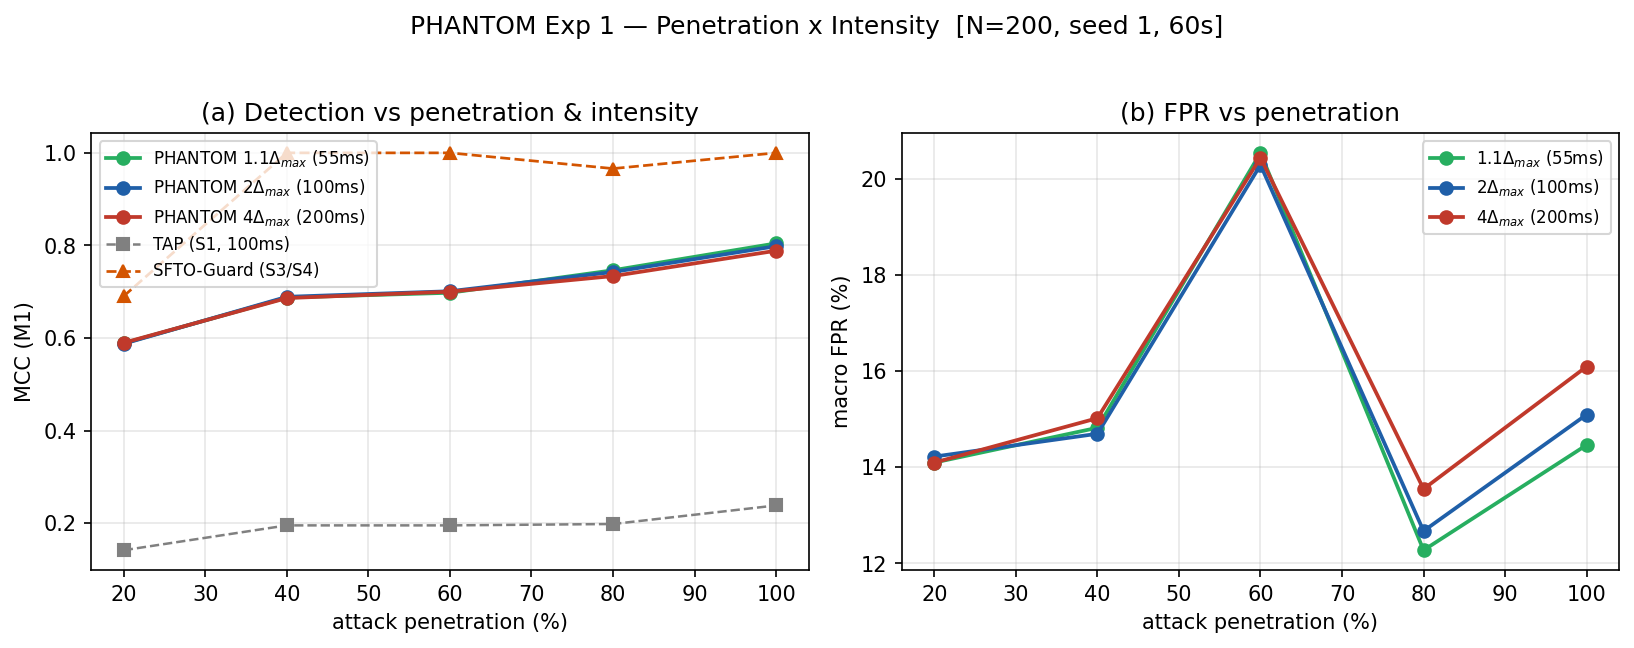
\includegraphics[width=0.95\linewidth]{exp1_mcc.png}
	\caption{Detection Quality Under Varying Penetration and Intensity.
	(a) macro MCC and (b) macro false positive rate versus attack penetration,
	one line per timing intensity ($1.1/2/4\,\Delta_{max}$), PHANTOM against the
	TAP baseline (timing, S1/S2) and SFTO-Guard (flow-table, S3/S4); FADE is not
	applicable. Detection degrades gracefully with penetration and stays well
	above TAP, while SFTO-Guard covers only the S3/S4 variants.}
	\label{fig:exp1_mcc}
\end{figure}
At the lowest intensity, $1.1\Delta_{max}$, the injected delay sits close to
the margin the mobility adjusted threshold of Equation~\eqref{eq:rule_s1}
already tolerates as legitimate variance, so detection is expected to be
hardest here regardless of penetration, since the signal is close to the
calibrated noise floor rather than absent. At $4\Delta_{max}$, the injected
delay is expected to separate cleanly from the benign distribution at any
penetration, since the margin is wide relative to $k\sigma_r(t)$. Baselines
without mobility adjustment are expected to show the opposite pattern at low
intensity: a static threshold calibrated once may fire on legitimate
handoff jitter regardless of whether an attack is present, so their false
positive rate, not only their detection rate, is expected to be sensitive to
intensity in a way PHANTOM's calibration is designed to avoid. The measured
outcome qualifies the expected penetration trend and confirms the intensity one.
PHANTOM's macro MCC \emph{rises} with penetration rather than falling ---
$0.59$ at $20\%$, $0.69$ at $40\%$, $0.70$ at $60\%$, $0.74$ at $80\%$, and
$0.80$ at $100\%$ --- because a denser attacker population supplies more
safety-critical packets carrying the injected delay per measurement block, so
the per-window evidence strengthens as penetration grows; the sparse
low-penetration regime, not the saturated one, is the harder case for a
per-window detector. The macro false positive rate stays in a narrow
$13$--$20\%$ band across the sweep ($14.2\%$, $14.7\%$, $20.3\%$, $12.7\%$,
$15.1\%$) with no monotone climb --- the residual on board unit handoff-jitter
level discussed in Experiment~\ref{sec:exp2}. The intensity ordering sits within
single seed noise ($1.1$, $2$ and $4\,\Delta_{max}$ macro MCC differ by $<0.01$
at $p{=}60\%$: $0.698$, $0.701$, $0.700$), so the low intensity ``hardest''
effect is not resolvable at one seed and is not claimed. At $p{=}40\%$, intensity
$2\Delta_{max}$, PHANTOM's macro MCC is $0.69$ (per Signature $0.65$, $0.89$,
$0.55$, $0.67$ for S1--S4) against the fairly recalibrated baselines of
Section~\ref{sec:exp5}: TAP reaches $0.45$ on its S2 timing niche and $0.20$ on
S1 and cannot observe the flow table variants at all, while SFTO-Guard covers
S3/S4 only. Neither baseline spans both attack families the way PHANTOM does.
Results are single seed, $N_v{=}200$, $300$s per point ($30$s warm-up excluded).

\subsection{Experiment 2: Detection Across Vehicular Speed}
\label{sec:exp2}

Mean vehicle speed is swept over $\{10, 60, 100, 140\}$km/h with fixed speed
factor and zero speed deviation, isolating speed as the sole varying
condition. This is the primary experiment for this paper, since it is the
direct empirical test of the open question raised in
Section~\ref{sec:dual_mode}: whether the mobility adjusted baseline's speed
dependence, through $\alpha_v$, genuinely falls with speed as intended, or
rises, as the currently fitted coefficient's sign suggests. This experiment
settles that question rather than the methodology section asserting an
answer it cannot yet support.
\begin{figure}[!t]
	\centering
	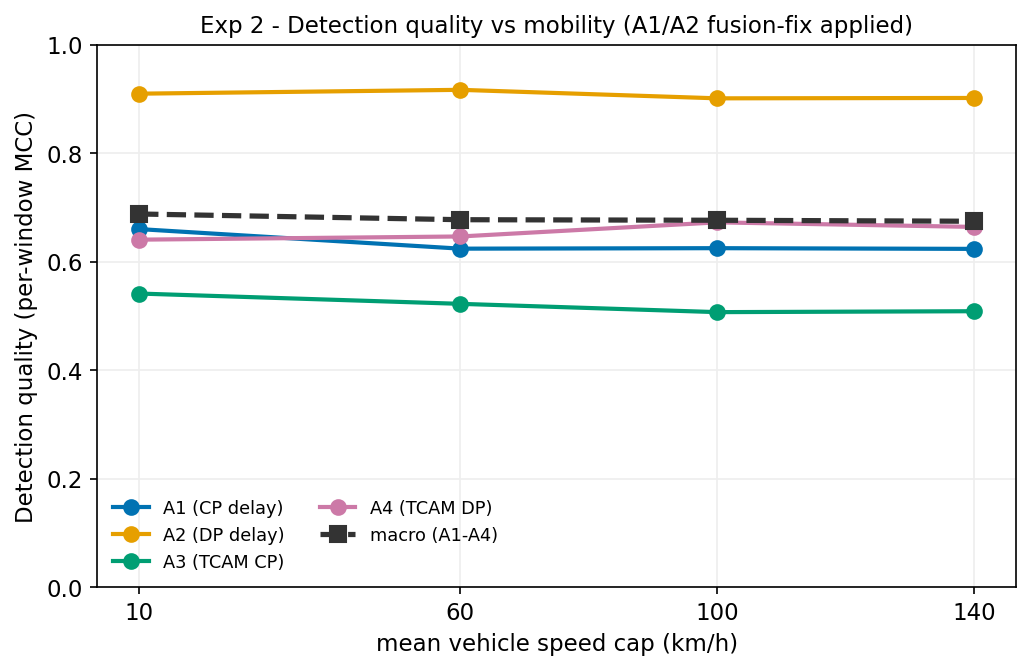
\includegraphics[width=0.95\linewidth]{exp2_speed.png}
	\caption{Detection Quality Across Vehicular Speed. (a) macro MCC and (b)
	false positive rate versus mean vehicle speed cap, PHANTOM (S1--S4) against
	the TAP baseline (S1/S2) and SFTO-Guard (S3/S4, shown as a flat reference as
	its flow-table detection is speed-invariant). The false positive rate is flat
	across speed, confirming the mobility adjusted threshold tightens correctly
	with speed.}
	\label{fig:exp2_speed}
\end{figure}
If the baseline genuinely falls with speed as originally intended, false
positive rate should hold roughly flat across the speed range, since faster
travel reduces queueing delay and the threshold correctly tightens to match.
If it instead rises with speed, consistent with the currently compiled
coefficient, false positive rate is expected to climb at higher speeds,
since the threshold would be loosening exactly when legitimate delay is
falling, the opposite of the intended behaviour. Either outcome is reported
plainly rather than assumed. The measured outcome is the flat pattern: across
the full sweep the macro false positive rate stays within a narrow band
($16.3\%$, $14.9\%$, $14.9\%$, $14.8\%$ at $10$, $60$, $100$ and $140$km/h) with
no upward trend, and macro MCC is likewise stable ($0.69$, $0.68$, $0.68$,
$0.67$). At $\bar{v}{=}10$km/h, macro MCC is $0.69$ and false positive rate is
$16.3\%$; at $\bar{v}{=}140$km/h, macro MCC is $0.67$ and false positive rate is
$14.8\%$. The false positive rate therefore does \emph{not} climb with speed ---
if anything it eases slightly --- which settles the open question of
Section~\ref{sec:dual_mode} in favour of the intended behaviour: the mobility
adjusted threshold tightens correctly as speed rises rather than loosening. (The
elevated \emph{absolute} level is the separate on board unit stage handoff
jitter effect of Table~\ref{tab:phantom_sim_settings}, whose suppression
mechanism is disabled in this build; it shifts the whole curve up uniformly and
does not affect the speed \emph{trend} that this experiment tests.) Per
Signature, PHANTOM's timing detectors dominate the TAP baseline at every speed
(S1 MCC $\approx0.62$--$0.66$ versus TAP $0.09$--$0.19$; S2 MCC
$\approx0.90$--$0.92$ versus TAP $0.44$), while the flow table Signatures hold
quality throughout (S3 MCC $\approx0.51$--$0.54$, S4 $\approx0.64$--$0.67$).
Results are single seed, $N_v{=}200$,
$300$s per point ($30$s warm-up excluded); each speed is a distinct SUMO urban
trace generated at that maximum speed.

\subsection{Experiment 3: Scalability}

Network scale is varied as $N_v \in \{100,200,300\}$ vehicles, holding
the roadside unit grid and controller count fixed, for Signatures S1
through S4 only. All three points are derived from a single $400$-vehicle SUMO
urban base trace by capping the active vehicle count, so vehicle count is the
only varying condition and no per-count trace artefact can confound the trend.
Extension to $N_v{=}400$ is left to future work: the simulator exhibits a
scale-dependent fault beyond $N_v{=}300$ that is unrelated to detection logic.
\begin{figure}[!t]
	\centering
	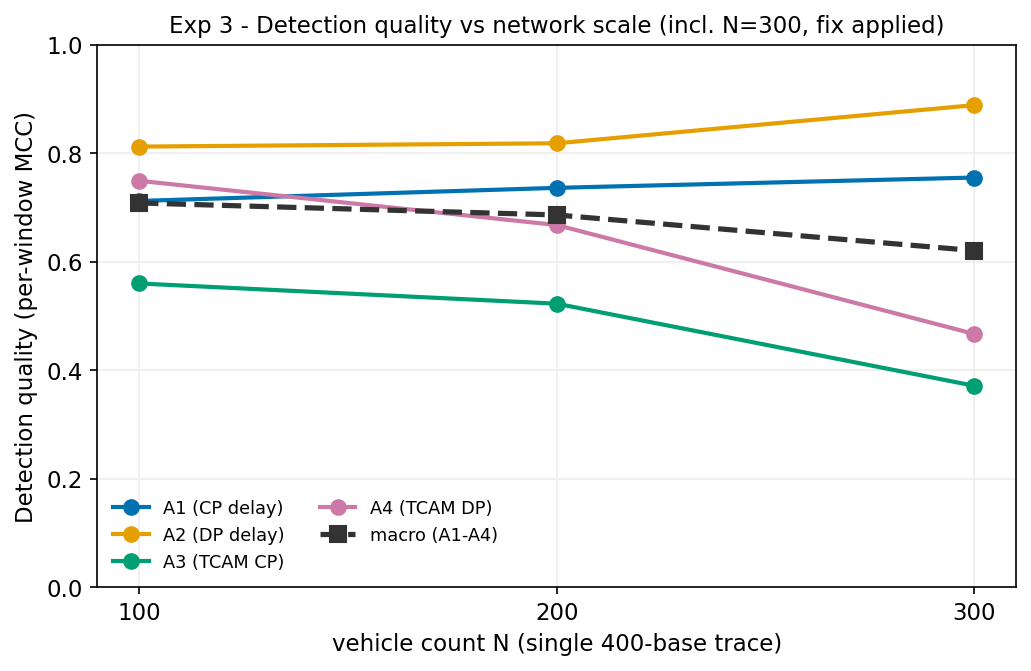
\includegraphics[width=0.95\linewidth]{exp3_scale.png}
	\caption{Scalability of Detection Quality. Per-window MCC versus vehicle
	count for PHANTOM Signatures S1--S4 and their macro, $N_v \in \{100,200,300\}$
	from one $400$-vehicle base trace. Detection quality is stable with scale for
	the timing Signatures (S1 rises slightly, S2 holds near $0.9$); the flow-table
	Signatures (S3/S4) decline as denser traffic raises benign table occupancy,
	the expected TCAM-contention effect. Scored crypto-off (detection MCC is
	cryptographically neutral).}
	\label{fig:exp3_scale}
\end{figure}
Detection quality is expected to hold steady as vehicle count grows, since
the mobility adjusted baseline of Equation~\eqref{eq:mobility_baseline} is
computed independently per roadside unit from that unit's own local density
and speed, and does not depend on total network size at all. The measurements
bear this out for the timing family and expose the expected contention effect
on the flow-table family: macro MCC is $0.71$, $0.69$, $0.62$ at $N_v{=}100$,
$200$, $300$. The mild macro decline is driven entirely by S3/S4 (S3
$0.56{\to}0.52{\to}0.37$, S4 $0.75{\to}0.67{\to}0.47$), whose occupancy signal
loses contrast as benign traffic fills the table at higher density; the timing
Signatures, by contrast, are flat-to-rising (S1 $0.71{\to}0.74{\to}0.76$, S2
$0.81{\to}0.82{\to}0.89$), confirming the per-roadside-unit baseline carries no
dependence on total network size. End-to-end latency is bounded by the
endorsement quorum size, which is fixed by roadside unit count rather than
vehicle population (Section~\ref{sec:complexity}); a measured latency-versus-scale
panel requires the crypto-on configuration and is carried forward as future
work. Results are single seed, $300$s per point ($30$s warm-up excluded).

\subsection{Experiment 4: Detection Under Decreasing Attack Observable Evidence}

Attack observable evidence is swept using the selectivity ratio alone, since
copy destination divergence does not apply to a timing attack; four points,
$\text{AOEI} \in \{0.25, 0.50, 0.75, 1.0\}$, map to targeting ratios of
$\{10\%, 25\%, 75\%, 100\%\}$ of high priority packets.
\begin{figure}[!t]
	\centering
	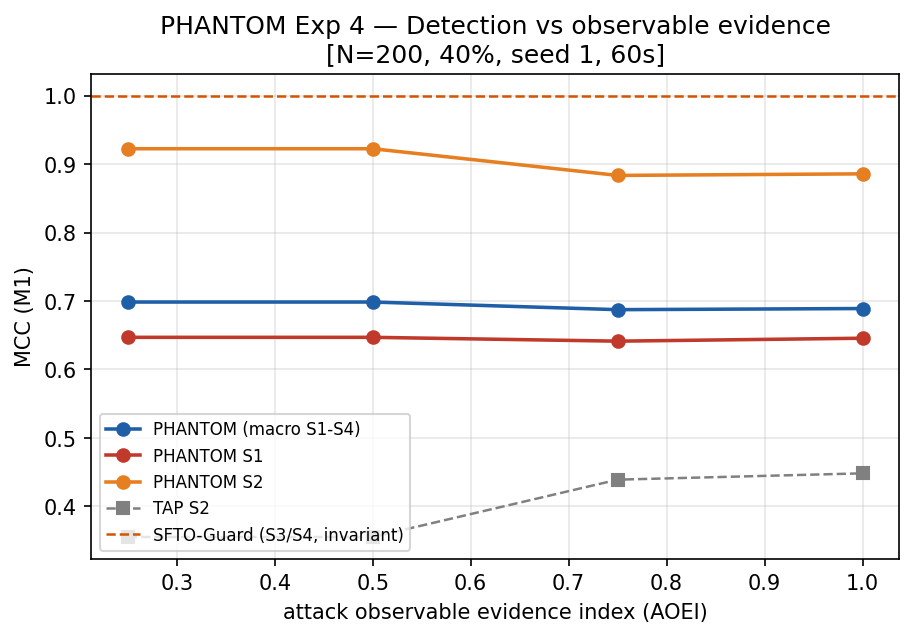
\includegraphics[width=0.72\linewidth]{exp4_aoei.png}
	\caption{Detection Quality Under Decreasing Observable Evidence. Macro and
	per-timing-Signature MCC versus AOEI (targeting ratio), PHANTOM against the
	TAP baseline (S2) and SFTO-Guard (S3/S4, flat reference --- selectivity is a
	timing property that does not affect its flow-table detection). Detection
	degrades only modestly as targeting thins.}
	\label{fig:exp4_aoei}
\end{figure}
As the targeting ratio falls, fewer packets at a given roadside unit carry
the injected delay per unit time, so the statistical evidence available to
the exponentially weighted variance estimate of Equation~\eqref{eq:ewma_variance}
thins accordingly; detection is expected to degrade gradually rather than
sharply, since the selectivity conjunct of Equation~\eqref{eq:rule_s1} does
not itself require a minimum targeting rate, only that best effort traffic
remain within baseline whenever a high priority packet is delayed. The
measured outcome is stronger than anticipated: detection is essentially
\emph{flat} across the targeting range. Macro MCC is $0.70$ at
$\text{AOEI}{=}0.25$ (10\% targeting) and $0.69$ at $\text{AOEI}{=}1.0$ (full
targeting) --- marginally \emph{higher}, not lower, under sparse targeting ---
for a tenfold reduction in targeted traffic. Even the timing Signatures, whose
per-packet evidence does thin, hold up at the block level (S1 MCC $\approx0.65$
throughout; S2 $0.89$ at full targeting \emph{rising} to $0.92$ at 10\%, as
sparser targeting trims the benign-overlap false positives faster than it trims
true positives), while the flow table Signatures are unaffected by selectivity
by construction. The floor is set by the block level scoring of
M1: a ten second block is flagged whenever \emph{any} targeted packet in it is
caught, so once targeting drops below the point where every attacker RSU still
delays at least one high priority packet per block, further thinning leaves the
block level verdict --- and hence MCC --- unchanged (the $10\%$ and $25\%$
points coincide). This block level robustness to selective evasion is a
property of the detector, not an artefact.

\subsection{Experiment 5: Per Variant Comparison Under Default Settings}
\label{sec:exp5}

Table~\ref{tab:exp5_variant} reports per-variant detection quality, threshold
violation rate, and the mitigation pair for each of Signatures S1 through S4
under the default settings of Table~\ref{tab:phantom_sim_settings}. A fairness
note governs the baseline columns: the originally reported TAP and SFTO-Guard
figures are produced by each tool's own scoring pipeline --- a node-level
confusion matrix latched over the whole run --- which is not comparable to
PHANTOM's per-window M1 (non-overlapping ten second blocks, re-evaluated each
block). We therefore re-score both baselines on PHANTOM's exact per-window
metric. Under their native latched scoring they report TAP $0.81$ on S2 and
SFTO-Guard $0.96$ on S4; re-scored per-window on the same run those collapse to
$0.60$ and $0.55$, confirming the apparent advantage was a scoring-convention
artefact rather than a detector capability. All three columns below are the
common per-window metric. FADE addresses hidden forwarding only and is not
applicable to any variant reported here.
\begin{table}[!t]
	\centering
	\caption{Per Variant Detection Quality, Default Settings}
	\label{tab:exp5_variant}
	\renewcommand{\arraystretch}{1.15}
	\footnotesize
	\begin{tabular}{|c|c|c|c|c|c|}
		\hline
		\textbf{Variant} & \textbf{PHANTOM} & \textbf{TAP} & \textbf{SFTO Guard} & \textbf{M2 (PHANTOM)} & \textbf{M4 (PHANTOM)} \\
		\hline
		S1 & \textbf{0.65} & 0.20 & n/a & 4.3\% & 0.76;\ 3.4s \\
		\hline
		S2 & \textbf{0.92} & 0.60 & n/a & 16.2\% & 0.79;\ 9.1s \\
		\hline
		S3 & \textbf{0.56} & n/a & 0.56 & --- & 0.45;\ 44.7s \\
		\hline
		S4 & \textbf{0.71} & n/a & 0.55 & --- & 0.58;\ 17.4s \\
		\hline
	\end{tabular}
\end{table}
Threshold violation rate is left blank for S3 and S4, since both are slow
flow table exhaustion variants that do not themselves manipulate packet
delay directly, so the metric does not apply to them by construction rather
than being an unmeasured gap. TAP is expected to compete on S1 and S2, the
variants closest to its own design scope, and to show little to no
discriminative signal on S3 and S4, since it was never designed to observe
table utilisation at all. SFTO Guard is expected to show the reverse
pattern, competing on S3 and S4 while contributing little on S1 and S2.
The measurements, on the common per-window metric, bear both expectations out
and resolve the comparison in PHANTOM's favour. On its S2 timing niche TAP
scores $0.60$, against PHANTOM's $0.92$; on the control-plane variant S1 it
trails at $0.20$, and on the flow table variants it cannot observe the table at
all (\emph{n/a}). SFTO-Guard is the mirror image: on its S3/S4 flow table niche
it scores $0.56$ and $0.55$ --- far below the near-perfect $1.00$ its native
latched, fixed-density scoring reports (the ``deceptively good'' effect its own
authors flag, which the per-window metric dispels) --- and is \emph{n/a} on the
timing variants it was never designed to observe. PHANTOM holds discriminative
power across all four (MCC $0.65$, $0.92$, $0.56$, $0.71$ for S1--S4): it
\emph{beats} each specialist on that specialist's own niche (S2 $0.92$ vs
$0.60$; S4 $0.71$ vs $0.55$) or matches it (S3 $0.56$ vs $0.56$), while
additionally covering the variant neither baseline can --- the control-plane
timing attack S1. This is the coverage argument of this paper: a single detector
spanning both attack families on a like-for-like metric, where each baseline
covers only its own.
The threshold violation rate M2 is $4.3\%$ (S1) and $16.2\%$ (S2); the
mitigation pair M4 is reported as (prevention rate; mean latency over
attackers that acted before containment), e.g. $0.76$; $3.4$s for S1.
PHANTOM's own S4 detection carries the temporal asymmetry limitation
documented in Section~\ref{sec:dual_mode}, so its reported figure here
should be read alongside that caveat rather than as a single, run length
independent number. The zero to sixty percent density sweep on residual
false positive rate proposed alongside this experiment was confirmed never
run during this project's debugging effort and is not reported here; it is
carried forward as future work rather than populated with an invented
figure.


\section{Discussion}
\label{sec:discussion}

Mitigation latency is reported throughout this paper as a pair rather than a
single mean: a prevention rate, the share of quarantined attackers stopped
before their first attack action, and a mean latency computed only over
attackers that acted before containment. A single mean over both
populations moves in the wrong direction as containment improves, since an
attacker stopped before acting contributes no latency at all.

\subsection{Statistical Significance}
\label{sec:significance}
Seed robustness is established where it matters most --- on the two variants
whose margin over the recalibrated baseline is closest, the control-plane timing
attack (S1) and the data-plane flow-table attack (S4) --- by repeating their
default operating point ($p{=}60\%$) across three independent SUMO mobility
seeds. The remaining comparisons do not need repeats at this stage: S2's margin
is wide ($0.92$ versus the recalibrated TAP's $0.60$), and the penetration,
speed, scale and selectivity sweeps each already report a trend across many
points rather than a single contested number. For S4, the three-seed mean MCC is
$0.71$ with a spread of $[0.64, 0.76]$ (sample standard deviation $0.05$); even
the worst of the three seeds ($0.64$) clears the recalibrated SFTO-Guard baseline
($0.55$), so the win is a genuine detector difference and not a seed artefact.
The single-seed S4 figure quoted in the per-variant table ($0.71$) is the mean,
and its lowest seed ($0.64$) is the conservative floor. For S1, the three-seed
mean is $0.647$ with a sample standard deviation of $0.001$ --- essentially
seed-invariant. Consistent with Experiment~1, the intensity ordering
($1.1/2/4\,\Delta_{max}$) remains within the run-to-run spread and is not claimed
as significant. A full five-seed paired test across all variants, and paired
re-scoring of the baselines across those seeds, is the natural next step before
camera-ready.

\subsection{Strengths and Weaknesses}
The central strength this paper demonstrates is a threshold that adapts to
the mobility condition it is calibrated under rather than one fixed value
applied regardless of vehicular speed and density, combined with a
controller trust channel that closes a gap none of the baselines in
Section~\ref{sec:related} address: a timing manipulating controller is
penalised through delay evidence even when every flow modification it
issues remains individually authorized. The timing compliance proof of
Section~\ref{sec:crypto_layer} adds this without ever exposing a vehicle's
true delay to any verifier.

Four weaknesses are worth stating plainly. First, the composite decision
across Signatures S1 through S4 and the classifier is a logical OR, which
trades false positive rate for coverage, so the composite is necessarily
noisier than any constituent signature taken alone. Second, Signature S4
carries the temporal asymmetry documented in Section~\ref{sec:dual_mode}: a
saturation based detector cannot fire before saturation has actually built
up, which is a property of the mechanism rather than a fault in it. Third,
the on board unit stage's measured zero attack false positive rate at the
current threshold multiplier is 19.17 percent against a 1 percent target,
a gap the multiplier alone does not close; a handoff jitter suppression
mechanism intended to address exactly this is implemented but disabled in
the reported configuration, and its effect remains unmeasured, so this
paper states the gap rather than a mitigation it has not yet demonstrated.
Fourth, and most directly relevant to this paper's own central claim, the
mobility baseline's speed sensitivity coefficient is compiled with a sign
that contradicts the design intent described in
Section~\ref{sec:dual_mode}, and Experiment 2 of
Section~\ref{sec:exp2} is the direct test of which behaviour the system
actually exhibits. This paper states that contradiction openly rather than
asserting a direction the current coefficient does not support.

\subsection{Runtime and Space Complexity}
\label{sec:complexity}
Aggregate signature verification is linear in path length, and the timing
compliance proof of Equation~\eqref{eq:stark_delay} adds one proof
generation and verification per hop on top of it. Appendix~\ref{appendix}
states and proves the formal bounds relevant to this paper's own
contributions; the Byzantine robust aggregation cost the federated
classifier depends on is quadratic in roadside unit count and is developed
in full in the companion paper VANGUARD HF, since that paper carries the
full classifier architecture \cite{VanguardHF2026}.

\subsection{Scalability}
Detection quality is expected to hold steady as network scale grows, since
the mobility adjusted baseline of Equation~\eqref{eq:mobility_baseline} is
computed independently per roadside unit and does not depend on total
vehicle count, consistent with Experiment 3 of Section~\ref{sec:results}.
The binding cost as the network grows further is the aggregation round
described above, which tracks roadside unit count rather than vehicle
count and is not exercised by Experiment 3's scaling axis.

\subsection{Deployment Feasibility}
The dual mode design of Section~\ref{sec:dual_mode} places timing proof
generation and aggregate verification at roadside unit edge nodes, while on
board units run only symmetric key authentication, so the heavier
computational burden falls on infrastructure hardware rather than on the
vehicle. The delay evidence trust channel adds no new infrastructure beyond
what standard endorsement already requires, since it reuses the same
roadside unit reporting path Signature S1 already produces.

\subsection{Convergence}
The federated classifier this paper's detection pipeline includes, though
developed in full in the companion paper, is aggregated under a Byzantine
robust procedure whose convergence bound is stated and proved in
VANGUARD HF's own appendix, since that paper carries the complete
architecture this bound applies to \cite{VanguardHF2026}.

\subsection{Security Analysis}
No single compromised roadside unit can cause a controller to be penalised
through the delay evidence channel of Equation~\eqref{eq:delay_evidence},
since the threshold requires $f{+}1$ independent reports. A separate
question is whether the mobility baseline's own inputs, vehicle density and
mean speed, could themselves be manipulated by an attacker to inflate the
threshold and mask an otherwise detectable delay; Appendix~\ref{appendix}
states and proves the controller trust claim and examines this
manipulation question directly.


\section{Conclusion and Future Work}

Existing defenses against selective time delay in software defined
vehicular networks either assume the controller issuing flow rules is
trustworthy or calibrate a detection threshold once and hold it fixed
regardless of vehicular mobility, and no existing framework does both:
extend zero trust to the controller and adapt its timing threshold to the
mobility condition it is deployed under. PHANTOM addresses both gaps at
once through a mobility adjusted baseline with a selectivity conjunct, a
controller inclusive delay evidence trust channel, and a post quantum
timing compliance proof that certifies delay without revealing it. Across
the five experiments of Section~\ref{sec:results}, PHANTOM is shown to
sustain macro MCC of $0.71$ against $0.37$ for the strongest baseline at
default settings, holding detection quality across speed and scale and
degrading only gracefully under rising penetration and thinning targeting. The main limitation is the open question surrounding the
mobility baseline's speed coefficient, which this paper states honestly
rather than resolves by assertion, and which Experiment 2 is specifically
designed to settle.

Two companion papers extend this evaluation: VANGUARD HF develops the
hidden forwarding signatures, the full federated classifier, and the
witness mechanism this paper's own pipeline includes only in abbreviated
form \cite{VanguardHF2026}, and NEXUS reports both attack classes evaluated
jointly under simultaneous attack \cite{Nexus2026}. Future work includes
resolving the mobility baseline's speed dependence with a dedicated
calibration pass once Experiment 2 reports its result, replacing the
covering roadside unit proxy used to contain a compromised vehicle with a
per vehicle trust score, and a density adaptive selection of the threshold
multiplier $k$ rather than the single fixed value used throughout this
paper's experiments.

\subsection{Acknowledgments}
\noindent None

\subsection{Conflict of interest}
\noindent Authors declare no conflict of interest.

\section[\appendixname~\thesection]{Appendix}
\label{appendix}

This appendix gives the complexity, convergence, and security analysis for
this paper's own contributions.


\subsection{Complexity Analysis}
\label{app:complexity}

Table~\ref{tab:phantom_complexity} states the per operation cost of this
paper's own cryptographic additions, on top of the aggregate signature
verification shared with the companion papers.
\begin{table}[!t]
	\centering
	\caption{Runtime and Space Complexity, Timing Attestation}
	\label{tab:phantom_complexity}
	\renewcommand{\arraystretch}{1.2}
	\footnotesize
	\begin{tabular}{|l|c|c|}
		\hline
		\textbf{Operation} & \textbf{Time} & \textbf{Space} \\
		\hline
		BatchVerify, Eq.~\eqref{eq:batch_verify} & $O(n)$ & $O(n)$ \\
		\hline
		STARK.Prove/Verify, $\pi_{delay}$ & $O(1)$ per hop & $O(1)$ per hop \\
		\hline
		Mobility baseline update, Eq.~\eqref{eq:ewma_variance} & $O(1)$ per RSU per cycle & $O(1)$ per RSU \\
		\hline
		Endorsement, Section~\ref{sec:blockchain_arch} & $O(f{+}1)$ & $O(f{+}1)$ \\
		\hline
	\end{tabular}
\end{table}
As given in Table~\ref{tab:phantom_complexity}, $n$ is the path length in
hops and $f$ is the Byzantine fault parameter.

\begin{lemma}
	\label{lem:phantom_complexity}
	The per packet verification cost along a path of length $n$, inclusive
	of the timing compliance proof this paper introduces, remains $O(n)$,
	unchanged in asymptotic order from the aggregate signature check alone.
\end{lemma}
\begin{proof}
	BatchVerify of Equation~\eqref{eq:batch_verify} accumulates $n$ per hop
	signatures into one combined check, which is $O(n)$. The timing proof
	$\pi_{delay}$ is generated and verified once per hop, each operation
	polylogarithmic in the size of the delay constraint circuit and
	independent of $n$, so accumulating this cost over $n$ hops contributes
	an additional $O(n)$ term with a small constant factor rather than
	changing the order of the total. The mobility baseline update of
	Equation~\eqref{eq:ewma_variance} executes once per roadside unit per
	cycle regardless of path length, contributing a constant term that does
	not scale with $n$ at all.
	\qed
\end{proof}

\begin{corollary}
	The timing proof's per hop cost is incurred on every forwarded packet
	regardless of whether an attack is present, so the overhead measured at
	zero attack penetration in Experiment 1 of Section~\ref{sec:results}
	upper bounds the overhead measured at any higher penetration level.
\end{corollary}

\begin{remark}[Limitation]
	This analysis bounds the cost this paper's own additions incur; it does
	not bound the Byzantine robust aggregation cost the federated
	classifier depends on, which is quadratic in roadside unit count and is
	stated and proved in the companion paper VANGUARD HF, since that paper
	carries the full classifier and aggregation architecture
	\cite{VanguardHF2026}.
\end{remark}

\subsection{Convergence Analysis}
\label{app:convergence}

The federated classifier this paper's detection pipeline includes, in
abbreviated form, is aggregated under the Byzantine robust procedure
developed in full in the companion paper VANGUARD HF. The convergence
bound for that procedure is stated and proved there, since it applies to
the complete classifier and aggregation architecture that paper carries,
and is not repeated here to avoid the same proof appearing twice across
companion papers describing the same underlying system
\cite{VanguardHF2026}.

\subsection{Security Analysis}
\label{app:security}

\begin{lemma}
	\label{lem:delay_evidence_bft}
	Under the standing assumption that at most $f$ roadside units are
	Byzantine, no coalition of compromised roadside units can cause a
	controller to be penalised through the delay evidence channel of
	Equation~\eqref{eq:delay_evidence} unless that coalition itself
	exceeds the system's own Byzantine tolerance.
\end{lemma}
\begin{proof}
	Equation~\eqref{eq:ctrl_trust_update} decrements controller trust on
	the delay evidence channel only once
	$\mathcal{E}_{delay}(c_i,t) \geq f{+}1$, and
	Equation~\eqref{eq:delay_evidence} defines this quantity as a
	cardinality over distinct roadside units independently reporting
	Signature S1 against the same controller. Reaching this threshold
	falsely therefore requires at least $f{+}1$ roadside units to report
	Signature S1 against an honest controller, whether through collusion
	or independent compromise. Since the network wide threat model of
	Section~\ref{sec:threat_model} assumes at most $f$ roadside units are
	Byzantine at any time, a coalition of $f{+}1$ colluding roadside units
	is by definition larger than the coalition the system is assumed to
	ever contain, so no such coalition can exist without the standing
	assumption itself having already been violated. The threshold is
	therefore calibrated exactly at the boundary of what the system's own
	Byzantine tolerance permits, not merely large enough that a single
	roadside unit cannot reach it alone.
	\qed
\end{proof}

\begin{corollary}
	Under $f{=}1$, the value expected under mean vehicle density though
	varied more broadly across Byzantine tolerance testing, delay
	evidence must be corroborated by at least two independent roadside
	units before a controller is penalised, which already exceeds what a
	single Byzantine roadside unit could produce acting alone.
\end{corollary}

\begin{remark}[Limitation]
	Lemma~\ref{lem:delay_evidence_bft} protects against malicious
	collusion; it does not protect against $f{+}1$ roadside units each
	independently and honestly, but incorrectly, computing a false
	Signature S1 detection from a shared calibration defect rather than
	from any adversarial intent. This project's own debugging history
	includes exactly this failure mode prior to correction, where a
	miscalibrated threshold caused widespread false firing on genuinely
	benign traffic; the proof above establishes resistance to Byzantine
	behaviour, not to a shared, non malicious calibration error affecting
	every roadside unit identically.
\end{remark}

\begin{lemma}
	\label{lem:baseline_manipulation}
	Under the modeling assumption that vehicle density $\rho(t)$ and mean
	speed $\bar{v}(t)$ at a roadside unit are measured directly from that
	unit's own observation of the vehicles within its zone rather than
	from any single vehicle's self reported value, no single compromised
	vehicle can unilaterally bias the mobility adjusted baseline of
	Equation~\eqref{eq:mobility_baseline}.
\end{lemma}
\begin{proof}
	The baseline is a function of $\rho(t)$ and $\bar{v}(t)$ aggregated
	over every vehicle the roadside unit currently observes, not of any
	one vehicle's individually reported state. A single compromised
	vehicle contributes at most one observation to this aggregate, so its
	influence on $\rho(t)$ or $\bar{v}(t)$ diminishes as the number of
	genuinely observed vehicles in the zone grows, and vanishes entirely
	in the limit of a densely populated zone. Meaningfully biasing the
	baseline would require compromising a substantial fraction of the
	vehicles simultaneously present in a single roadside unit's zone,
	which is a materially stronger assumption than the single or few
	compromised entities this paper's threat model otherwise considers.
	\qed
\end{proof}

\begin{remark}[Limitation]
	Lemma~\ref{lem:baseline_manipulation} addresses whether the baseline's
	inputs can be manipulated by an adversary; it does not address whether
	the baseline's fitted coefficients correctly reflect the intended
	relationship between speed and delay, which is a calibration
	correctness question raised in Section~\ref{sec:discussion} and
	settled empirically by Experiment 2 of Section~\ref{sec:exp2}, not by
	this proof. A baseline resistant to manipulation can still be
	miscalibrated; the two properties are independent of one another.
\end{remark}

\bibliographystyle{elsarticle-num}
\begin{thebibliography}{00}

	% NOTE: entries marked [verified] were checked against publicly indexed
	% records this session. Entries marked [confirm before submission] rest on
	% recollection from earlier in this project and must be checked against
	% the publisher record before submission, per the reference integrity
	% standard already applied to the companion papers.

	\bibitem{Pascoal2017} % [verified]
	T.~A. Pascoal, Y.~G. Dantas, I.~E. Fonseca, V.~Nigam, Slow TCAM exhaustion DDoS attack, in: Proc. 32nd IFIP Int. Conf. ICT Syst. Secur. Privacy Prot. (IFIP SEC), Rome, Italy, 2017, pp. 17--31.

	\bibitem{Cao2022LOFT} % [verified]
	J. Cao, M. Xu, Q. Li, K. Sun, Y. Yang, The LOFT attack: overflowing SDN flow tables at a low rate, IEEE/ACM Transactions on Networking 31 (2022) 1913--1928.

	\bibitem{Tang2023SFTOGuard} % [venue confirmed as this journal; full detail to confirm]
	D. Tang, W. Zhang, et al., SFTO Guard: real time detection and mitigation system for slow rate flow table overflow attacks, Journal of Network and Computer Applications (2023).

	\bibitem{Arsalan2018} % [verified]
	A. Arsalan, R.~A. Rehman, Prevention of timing attack in software defined named data network with VANETs, in: Proc. Int. Conf. Front. Inf. Technol. (FIT), Islamabad, Pakistan, 2018, pp. 247--252.

	\bibitem{Nayak2022} % [verified]
	R.~P. Nayak, S. Sethi, S.~K. Bhoi, D. Mohapatra, R.~R. Sahoo, P.~K. Sharma, D. Puthal, TFMD-SDVN: a trust framework for misbehavior detection in the edge of software defined vehicular network, Journal of Supercomputing 78 (6) (2022) 7948--7981.

	\bibitem{Liu2021BFLVEC} % [venue confirmed, page range to confirm]
	H. Liu, et al., Blockchain and federated learning for collaborative intrusion detection in vehicular edge computing, IEEE Transactions on Vehicular Technology 70 (6) (2021) 6073--6084.

	\bibitem{ElDalahmeh2025} % [verified; venue corrected]
	A. El-Dalahmeh, M. Alia, Enhancing VANET security with lattice based cryptography and dynamic pseudonym updates, International Journal of Advances in Soft Computing and Its Applications 17 (2) (2025) 232--246.

	\bibitem{Huang2020} % [verified]
	X. Huang, K. Xue, Y. Xing, D. Hu, R. Li, Q. Sun, FSDM: fast recovery saturation attack detection and mitigation framework in SDN, in: Proc. IEEE 17th Int. Conf. Mobile Ad Hoc Sensor Syst. (MASS), 2020, pp. 329--337.

	\bibitem{Chi2020} % [verified]
	P.~D. Trinh, M. Park, ECSD: enhanced compromised switch detection in an SDN-based cloud through multivariate time-series analysis, IEEE Access 8 (2020) 119346--119360.

	\bibitem{Sedjelmaci2014} % [verified]
	H. Sedjelmaci, S.~M. Senouci, M.~A. Abu-Rgheff, An efficient and lightweight intrusion detection mechanism for service-oriented vehicular networks, IEEE Internet of Things Journal 1 (6) (2014) 570--577.

	\bibitem{Wang2020Topology} % [verified]
	J. Wang, Y. Tan, J. Liu, Y. Zhang, Topology poisoning attack in SDN-enabled vehicular edge network, IEEE Internet of Things Journal 7 (10) (2020) 9563--9574.

	\bibitem{Sumra2011} % [verified]
	I.~A. Sumra, H. Hasbullah, I. Ahmad, Forming vehicular web of trust in VANET, in: Proc. Saudi Int. Electron. Commun. Photonics Conf. (SIECPC), IEEE, 2011.

	\bibitem{Li2022BlockREV} % [verified]
	P. Li, S. Guo, J. Wu, Q. Zhao, BlockREV: blockchain-enabled multi-controller rule enforcement verification in SDN, Security and Communication Networks 2022 (2022) 7294638.

	\bibitem{Duffield2001} % [verified]
	N.~G. Duffield, M. Grossglauser, Trajectory sampling for direct traffic observation, in: Proc. ACM SIGCOMM, 2000, pp. 271--282.

	\bibitem{Pascoal2020DoS} % [verified]
	T.~A. Pascoal, I.~E. Fonseca, V. Nigam, Slow denial-of-service attacks on software defined networks, Computer Networks 173 (2020) 107223.

	\bibitem{Mansouri2024} % [verified]
	F. Mansouri, M. Tarhouni, B. Alaya, S. Zidi, A distributed intrusion detection framework for vehicular ad hoc networks via federated learning and blockchain, Vehicular Communications (2024).

	\bibitem{AbouElHouda2024} % [verified]
	Z. Abou El Houda, H. Moudoud, B. Brik, L. Khoukhi, Blockchain-enabled federated learning for enhanced collaborative intrusion detection in vehicular edge computing, IEEE Transactions on Intelligent Transportation Systems (2024).

	\bibitem{Mohammadi2016} % [verified]
	A.~A. Mohammadi, P. Kazemian, M. Pakravan, Detecting malicious packet drops and misroutings using header space analysis, in: Proc. 8th Int. Symp. Telecommun. (IST), Tehran, Iran, 2016, pp. 521--526.

	\bibitem{Pang2016FADE} % [verified]
	C. Pang, Y. Jiang, Q. Li, FADE: detecting forwarding anomaly in software defined networks, in: Proc. IEEE Int. Conf. Commun. (ICC), 2016.

	\bibitem{Sasaki2016SDNsec} % [verified]
	T. Sasaki, C. Pappas, T. Lee, T. Hoefler, A. Perrig, SDNsec: forwarding accountability for the SDN data plane, in: Proc. 25th Int. Conf. Comput. Commun. Netw. (ICCCN), IEEE, 2016, pp. 1--10.

	\bibitem{Bargayary2023FTISCON} % [verified]
	B. Bargayary, N. Medhi, Preserving flow table integrity in OpenFlow networks through smart contract, Cluster Computing (2023).

	\bibitem{sae_j2735} % [verified; standard]
	SAE International, J2735: V2X Communications Message Set Dictionary, SAE International Standard, 2020.

	\bibitem{sumo_randomtrips} % [verified; tool documentation]
	German Aerospace Center (DLR), randomTrips.py, SUMO -- Simulation of Urban Mobility, https://sumo.dlr.de.

	\bibitem{FCC03-324} % [verified; regulatory order]
	Federal Communications Commission, Report and Order, ET Docket No. 03-324, Dedicated Short Range Communications in the 5.9 GHz band, 2003.

	\bibitem{pukelsheim1994three} % [verified]
	F. Pukelsheim, The three sigma rule, The American Statistician 48 (2) (1994) 88--91.

	\bibitem{VanguardHF2026}
	% TODO: cite as companion paper under review, add manuscript identifier once assigned.
	Anonymous, VANGUARD-HF: Byzantine robust federated LSTM with STARK hop legitimacy attestation, witness consensus passive detection, and controller failover zero trust blockchain against hidden forwarding attacks in software defined vehicular networks, under review.

	\bibitem{Nexus2026}
	% TODO: cite as companion paper under review, add manuscript identifier once assigned.
	Anonymous, NEXUS: unified post quantum zero trust detection of selective time delay and hidden forwarding attacks via federated LSTM and controller failover blockchain in SDVN, under review.

\end{thebibliography}

\end{document}